%=============================================================================
%  Structural Influence: Measuring the Hidden Wiring of an NBA Offense
%
%  Build: pdflatex paper && bibtex paper && pdflatex paper && pdflatex paper
%  Figures: place fig1_wiring.png and fig5b_signatures.png in ./figures/
%=============================================================================
% !TEX program = pdflatex
\documentclass[11pt]{article}

\usepackage[margin=1in]{geometry}
\usepackage{amsmath,amssymb,amsthm}
\usepackage{bm}
\usepackage{booktabs}
\usepackage{graphicx}
\graphicspath{{figures/}{./}}
\usepackage{xcolor}
\usepackage{multirow}
\usepackage{array}
\usepackage{caption}
\usepackage{subcaption}
\usepackage{float} % [H] = place figure HERE, not at page end
\usepackage{placeins} % \FloatBarrier keeps floats inside their section
\usepackage{longtable} % appendix shaper roster table
\usepackage{needspace} % reserve vertical space before large floats
\usepackage{enumitem}
\usepackage[hidelinks]{hyperref}
\usepackage[numbers,sort&compress]{natbib}
\usepackage{tikz}
\usetikzlibrary{arrows.meta,positioning}

% ---- notation macros (single source of truth; do not redefine inline) -------
\newcommand{\Bmat}{\ensuremath{\bm{B}}} % player x play-type initiation matrix
\newcommand{\Amat}{\ensuremath{\bm{A}}} % play-type association matrix (invariant)
\newcommand{\Afull}{\ensuremath{\Amat_{\text{full}}}}
\newcommand{\Aminus}[1]{\ensuremath{\Amat_{-#1}}}
\newcommand{\load}{\ensuremath{L}} % structural influence
\newcommand{\resid}{\ensuremath{r}} % usage-residual structural influence
\newcommand{\dA}{\ensuremath{\Delta\Amat}} % adjacency-displacement signature
\newcommand{\pt}{\ensuremath{\bm{\pi}}} % play-type profile
\newcommand{\cossim}{\operatorname{cos}}
\newcommand{\PPP}{\text{PPP}}
\DeclareMathOperator*{\argmax}{arg\,max}

\newtheorem{definition}{Definition}
\newtheorem{hypothesis}{Hypothesis}

\title{\textbf{Structural Influence: Measuring the Hidden Wiring of an NBA Offense}}

\author{Rami Zheman \\ Independent Researcher, Alexandria, VA}
\date{August 2026}

\begin{document}
\maketitle

%=============================================================================
\begin{abstract}
\noindent
NBA teams spend billions on players, yet some of the hardest to characterize are the ones who
shape how an offense operates. Box scores barely see them.
Existing analytics measure production, efficiency, and usage, but not how an offense is
organized, or how much its structure changes around any one player.

Teams' offensive organizations are mapped as a network representing players and the play types
they initiate. A player's structural influence is how much the graph's shape changes when he is
removed, meaning how much the offense reorganizes if that player were out. Crossing structural
influence against usage identifies low-usage players whose absence reorganizes the offense
comparable to losing a high-usage playmaker.

Using public data across three NBA seasons, this paper finds that a player's organizational
influence, after accounting for how much he touches the ball, is largely uncorrelated with
value metrics such as net rating. These players, referenced in this paper as shapers, instead
affect the team's offensive footprint.
On the floor, shapers typically mean teams run more cuts and pick-and-rolls and fewer spot-ups
and drives. Their structural influence partly travels with the player after a trade, affecting
a new team's offense too. High-usage organizational talent affects scoring efficiency reliably;
a shaper's structural influence does not. What an offense reorganizes around structurally is
not the same as what makes it score.

With this framework, researchers can study how an offense reorganizes when key players are
unavailable, coaches can prepare for in-game offensive pivots when players go out, and front
offices can see how much a trade or absence changes team identity. Offensive organization
becomes measurable, not just coaching intuition.
\end{abstract}
%=============================================================================
\section{Introduction}
\label{sec:intro}

\paragraph{A motivating problem.}
NBA teams spend enormous resources evaluating players, yet some of the hardest to assess
are those whose contribution is organizational. Coaches, teammates, and front offices
consistently describe ``glue guys'' who connect an offense, create opportunities for
others, or hold a system together, even when the box score grades them as rotation pieces
rather than difference-makers. At the February 2024 trade deadline, Dallas sent a
first-round pick to Washington for Daniel Gafford, a backup center averaging roughly
eleven points and eight rebounds, and reached the Finals with him starting at center. The
anecdote poses a clean question: \emph{what might a front office be buying that production,
efficiency, and usage metrics do not measure?}

Existing analytics answer how much a player contributes to winning
\citep{rosenbaum2004apm, sill2010winval} and what type of player he is
\citep{lutz2012cluster, alagappan2012positions}. They do not directly measure how an
offense is organized, or how dependent that organization is on any individual. This paper
is not about proving that glue guys are secretly stars, and it is not primarily about
whether organizational completeness raises points per possession. It asks a prior
question: whether \emph{offensive organization itself} can be measured.

\paragraph{Why measuring organization matters.}
Basketball analytics has become increasingly good at measuring outcomes. Offensive
organization remains one of the last major aspects of team performance that is still
largely qualitative, at both the player and the team level. A reproducible measure of
offensive wiring enables questions that outcome models leave unasked: how offenses
reorganize after injuries; which offenses are structurally \emph{brittle}, concentrating
their wiring in one or two players, versus distributed and resilient to any single
absence; how organizational responsibility changes as rookies develop; whether trades
preserve or rewire offensive identity; and, symmetrically, which defenders most disrupt an
opponent's wiring. None of these route through proving that any player is worth a fixed
number of extra points; they are decision-relevant questions about structure.
As shown below, that structure is largely independent of scoring efficiency itself
(Sec.~\ref{sec:efficiency}): what a front office would be buying is organizational
continuity, not points. Treating
organizational function as a measurable property rather than an anecdotal one expands the
scientific questions basketball analytics (and, more generally, the study of collaborative
systems) can ask. The contribution is the instrument. The empirical results below are what
that instrument reveals in a first confirmatory pass, not the only reason it matters.

\paragraph{Contribution A: a measurement framework.}
This paper first introduces a reproducible graph-based framework for measuring offensive
organization. An offense is represented as a bipartite player--play-type initiation graph.
Its \emph{wiring} is the team-level map of which players jointly hold which offensive
responsibilities. Each player's \emph{structural influence} is the change in that map when he is
removed: organizational dependence operationalized as network perturbation. Crossing influence
with usage isolates \textsc{Shaper} players (low usage, high residual influence), the
offensive face of the glue-guy folklore, not a census of defense, rebounding, or
intangibles. Gafford will return only as an illustration of that class, not as its
definition.

This is a graph problem because the scientific object is relational dependence, not a
player effect or an outcome. Existing statistical approaches primarily estimate how much a
player contributes to points or wins. The objective is different: quantify how the
\emph{relational organization} of an offense changes when a participant disappears. Graph
representations encode interactions among players and offensive actions explicitly, so
dependence can be measured by removing a node and observing reorganization, rather than
inferred indirectly from outcomes. This paper does not claim graphs are the only conceivable tool;
it argues they are the natural tool for this question, in the same sense that removing a
gene, an airport, or a power station is naturally a network-perturbation question.

\paragraph{Contribution B: what the framework reveals.}
This paper then uses the framework to study organizational function across three NBA seasons
(2022--23 through 2024--25). The remainder of the paper demonstrates what the measurement
reveals, in a fixed confirmatory order:
\begin{enumerate}[leftmargin=1.6em,itemsep=0.1em]
 \item \textbf{Does the measure reveal something new?} Low-usage players can carry
 organizer-level structural influence (Sec.~\ref{sec:emerge}).
 \item \textbf{Is it just another value metric?} Residual influence is essentially orthogonal
 to net rating (Sec.~\ref{sec:orthogonality}).
 \item \textbf{Does it correspond to observable basketball?} Shaper presence is
 associated with recognizable play-mix shifts (Sec.~\ref{sec:behavior}).
 \item \textbf{Where does the construct stop?} Completeness / shaper presence do not
 independently raise PPP beyond talent, a boundary finding: structural dependence is
 measurable, but not equivalent to offensive efficiency (Sec.~\ref{sec:efficiency}).
 \item \textbf{Does identity move when efficiency does not?} A disclosed post-hoc on/off
 test: shaper absence displaces the observed association fingerprint more than
 usage-matched role-occupant absence (Sec.~\ref{sec:identity-resilience}).
 \item \textbf{Is it partly player-specific?} A player-level component of organizational
 function persists across team changes on average, imperfectly, as a distribution
 (Sec.~\ref{sec:portability}).
 \item \textbf{Can transfer be predicted?} Destination vacancy is null under the
 measures tested; within shapers, origin cut vs.\ drive diet is a directional but
 exploratory, non-confirmed candidate (Sec.~\ref{sec:travelfit}).
\end{enumerate}

\paragraph{Same menu, different wiring.}
Figure~\ref{fig:wiring} makes the measurement target concrete. Minnesota and Houston in
2023--24 ran nearly identical offensive menus (menu cosine $0.99$) yet assigned
responsibilities differently (wiring cosine $0.54$). A possession table sees identical
menus; the graph sees different organization. This paper models shared initiators across play types
over a season, not within-possession sequence. The figure is only that demonstration.

\begin{figure}[H]
  \centering
  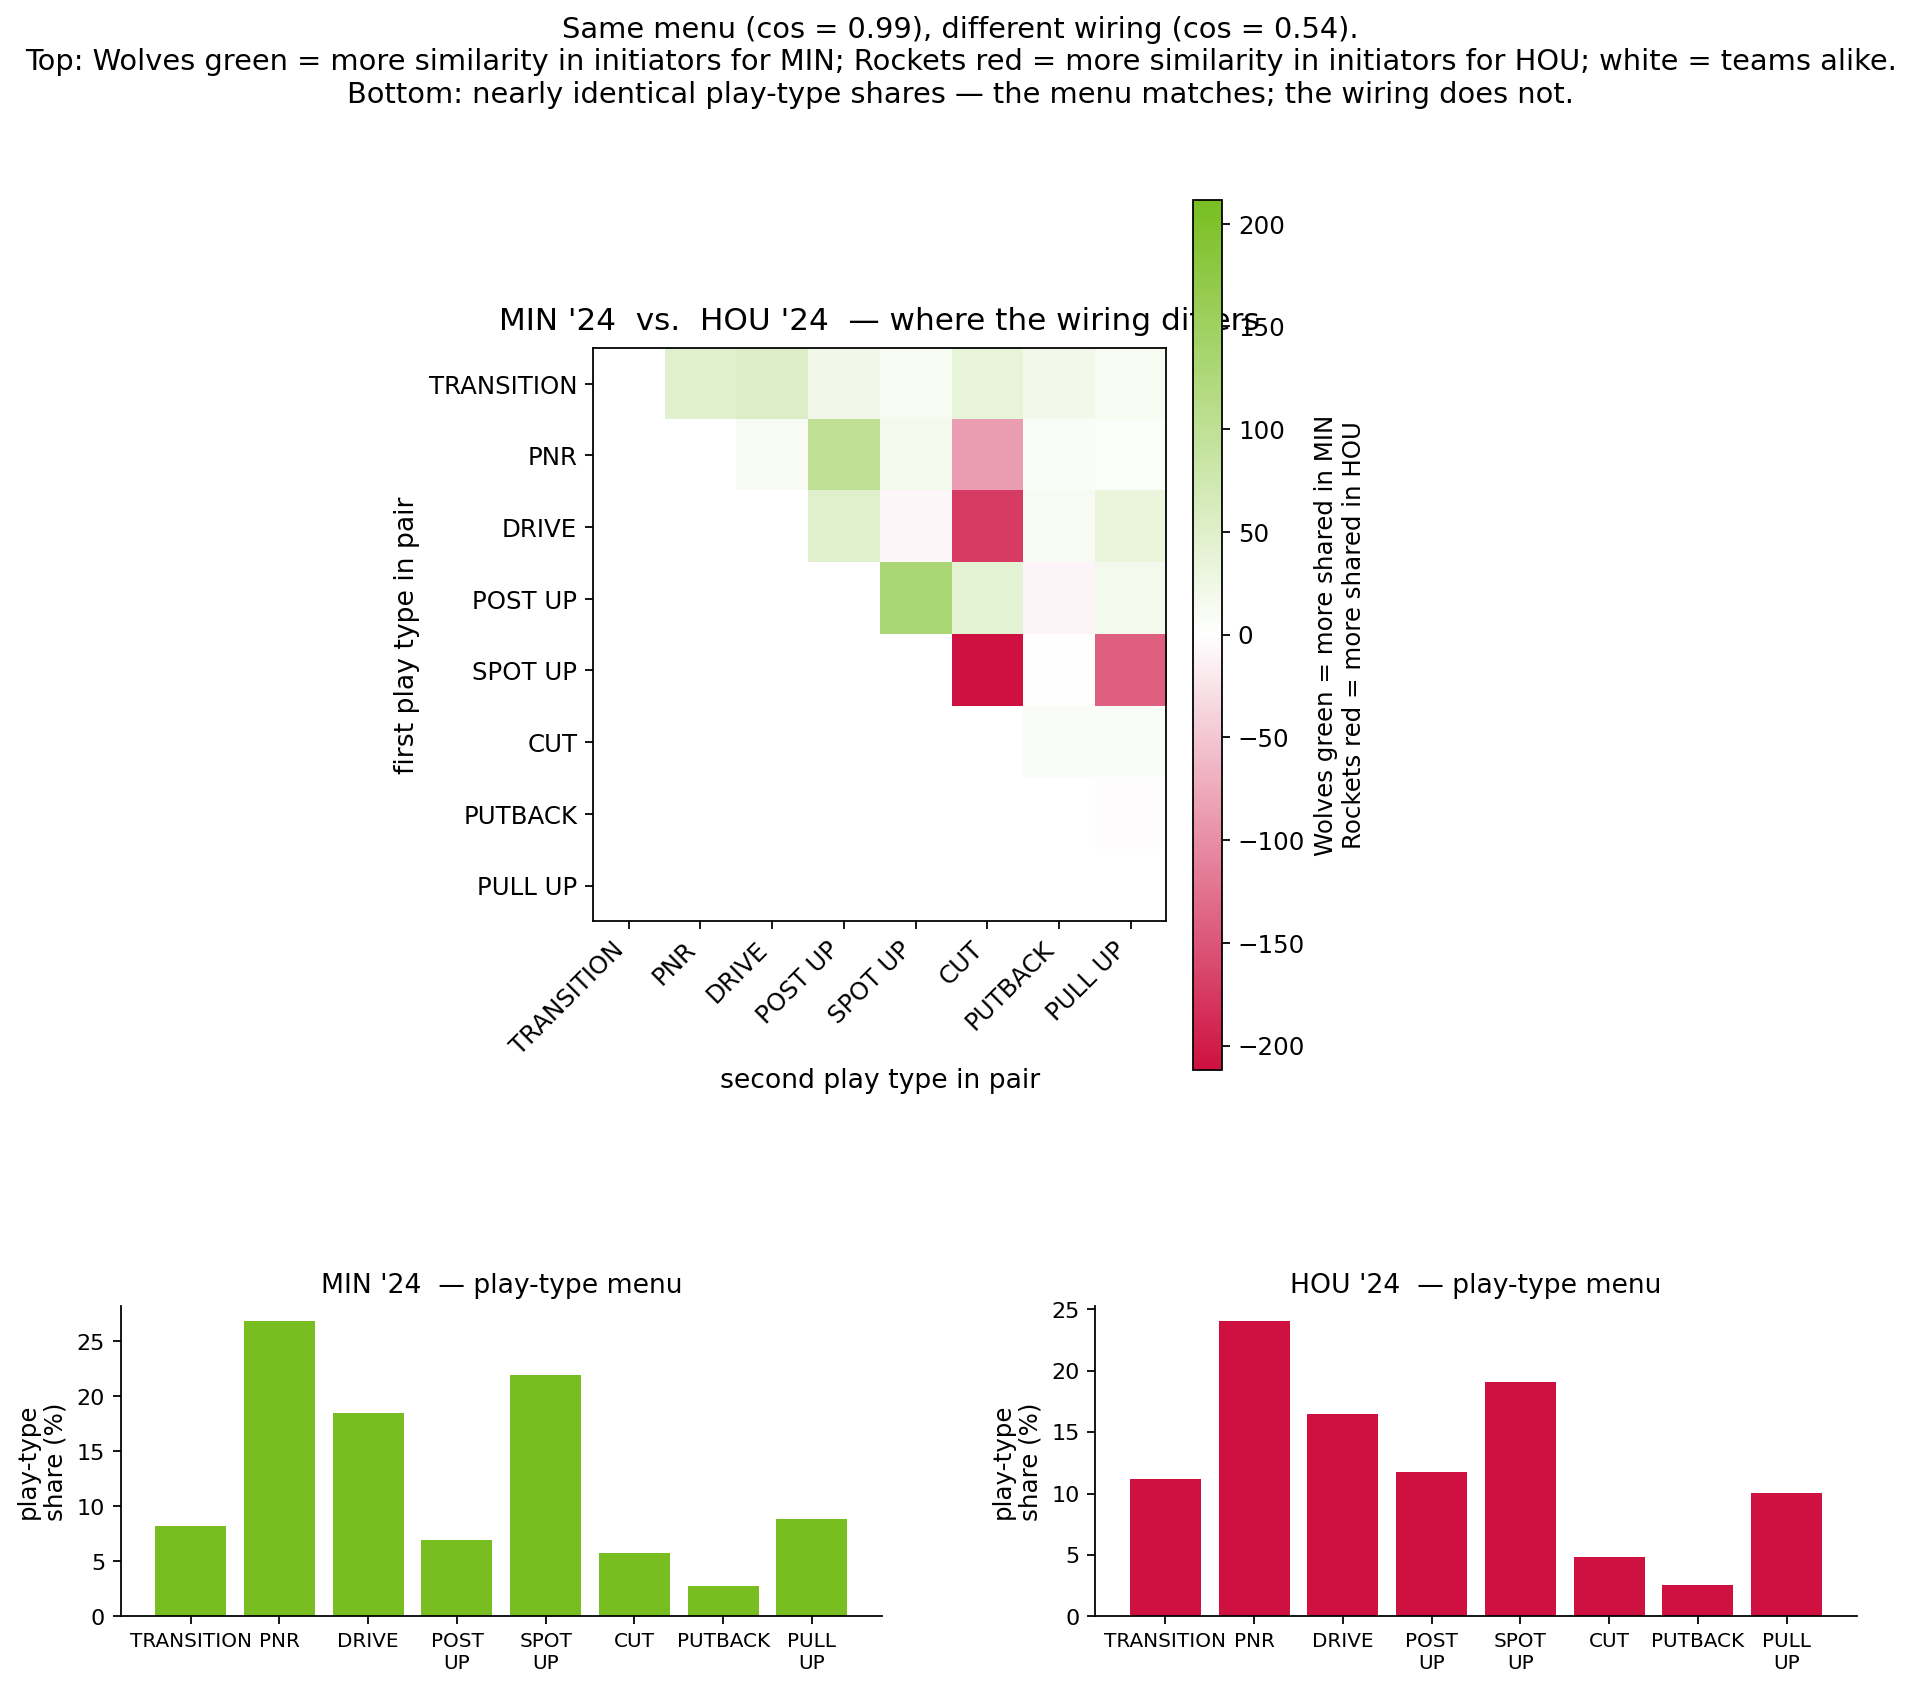
\includegraphics[width=\textwidth]{fig1_wiring.png}
 \caption{\textbf{Same menu, different wiring.}
 \textbf{(1) Bottom bars = the menu.} How often each team \emph{initiates} each play type
 (marginal frequency). Minnesota (MIN) and Houston (HOU) are nearly identical (cosine $0.99$).
 \textbf{(2) Top heatmap = where the responsibility maps differ.} Each cell is a play-type
 pair: shared-initiator score for Minnesota minus Houston (each first centered on its own team
 average). \textbf{Wolves green} $=$ more initiator overlap for Minnesota;
 \textbf{Rockets red} $=$ more for Houston; white $\approx$ teams alike.
 \textbf{Example:} POST\_UP--SPOT\_UP is green (Minnesota's post-up and spot-up initiators
 overlap more); DRIVE--CUT and SPOT\_UP--CUT are deep red. Same menu, different roster map.}
  \label{fig:wiring}
\end{figure}

\begin{figure}[H]
 \centering
 \begin{tikzpicture}[
 font=\small,
 box/.style={draw, rounded corners=2pt, align=center, inner sep=6pt,
 minimum width=4.0cm},
 step/.style={box, fill=black!6},
 arr/.style={-{Latex}, thick},
 ]
 \node[step] (s1) {\textbf{1. Measure:} wiring + structural influence};
 \node[step, below=5mm of s1] (s2) {\textbf{2. Validate:} not value; visible on floor};
 \node[step, below=5mm of s2] (s3) {\textbf{3. Bound:} no PPP premium beyond talent};
 \node[step, below=5mm of s3] (s3b) {\textbf{3b. Identity:} on/off fingerprint moves (post-hoc)};
 \node[step, below=5mm of s3b] (s4) {\textbf{4. Transfer:} does organizational function reappear?};
 \draw[arr] (s1) -- (s2);
 \draw[arr] (s2) -- (s3);
 \draw[arr] (s3) -- (s3b);
 \draw[arr] (s3b) -- (s4);
 \end{tikzpicture}
 \caption{\textbf{Paper spine.} Contribution~A builds the instrument. Contribution~B asks
 what it reveals: distinctness from value, behavioral correspondence, an efficiency
 boundary, a disclosed post-hoc identity follow-up, and imperfect portability
 (Secs.~\ref{sec:framework}--\ref{sec:travelfit}). Shapers are the visible stress-test
 subclass, not the paper's sole object.}
 \label{fig:spine}
\end{figure}

\paragraph{Central claim.}
Organizational function can be measured from initiation structure; it is not player value;
and it travels imperfectly. Players possess a measurable organizational function that is
distinct from talent, manifests in offensive behavior, and is partially player-associated
rather than entirely determined by team context. Shapers make hidden structural
dependence visible; they are not the paper's
sole object. Named movers (Gafford upper-tail, Delon Wright lower-tail) illustrate a
distribution; they do not define it.

%=============================================================================
\section{Related Work}
\label{sec:related}

\paragraph{Positions and archetypes.}
Efforts to modernize the five positions re-cluster players by box-score and shot-location
profiles into data-driven ``archetypes'' \citep{lutz2012cluster,alagappan2012positions}. These
describe \emph{what a player does with the ball} but remain player-marginal: they never model
how a player's actions relate to teammates' actions, and they do not ask whether a description
transfers between teams. Organizational function is defined by \emph{relational displacement}
(Sec.~\ref{sec:framework}); portability is exactly the transfer question archetypes leave open.

\paragraph{Player similarity and embeddings.}
A large literature embeds players for similarity search \citep{sill2010winval}. Such embeddings
answer ``who resembles this player?'' in feature space; they do not distinguish a transportable
property from a shared environment. That distinction (trait vs.\ artifact) is the pivot of
Contribution~B.

\paragraph{Lineup and value models.}
Plus/minus and its regularized descendants and five-man lineup net-rating analyses estimate
\emph{value} and identify \emph{which groups perform well} \citep{rosenbaum2004apm,
sill2010winval}. They are, by construction, silent on organizational function and on whether a
player's contribution is his to carry elsewhere. This paper positions organizational function
\emph{alongside} these models: it measures a different axis, and Sec.~\ref{sec:orthogonality}
and Sec.~\ref{sec:efficiency} confirm it does not add scoring beyond the talent they already
price.

\paragraph{Network analysis in basketball.}
Prior network work models passing as a graph and computes possession-level flow statistics,
notably ``the price of anarchy'' and centrality of ball movement \citep{fewell2012basketball,
skinner2010anarchy}. This establishes that graph representations are meaningful in basketball,
but the object is \emph{within-possession ball movement} and the target is \emph{team-level}
flow efficiency. This paper differs in object and question: play-type co-initiation graphs at the
\emph{team-season} level, a \emph{player-level} measure of organizational dependence via
node-removal perturbation, and a test of whether that function contains a portable
player-level component.

\paragraph{The gap.}
Across positions, archetypes, embeddings, lineup models, and passing networks, the field
has tools for \emph{value}, \emph{activity}, and \emph{flow}, but none that measures an
offense's wiring as a team-level responsibility map, identifies players on whom that
wiring depends through network perturbation, or tests whether a player's ability to wire
an offense together persists across team changes. That gap is what this paper addresses.

% RECOMMENDED TABLE (Table 1, end of Related Work):
%   A "capability matrix": rows = {positions, archetypes, embeddings,
%   lineup/value models, passing networks, OURS}; columns = {measures value?,
%   measures activity?, measures relational structure?, player-level?,
%   tests portability?}. Checkmarks make the gap visually obvious :  only OURS
%   checks "relational structure" AND "tests portability".

%=============================================================================
\section{Data}
\label{sec:data}

\paragraph{Source and unit.}
The data are possession-level records for three NBA regular seasons
(2022--23, 2023--24, 2024--25). The atomic unit is a \emph{possession}, annotated with the
offensive and defensive team, the initiating player, the possession's \emph{play type}, the
points scored, and contextual fields (period, score margin, and, for the subset of seasons
with on-court tracking, the five offensive players on the floor). After restricting to
possessions with a resolved initiator and a play type in the canonical set, the corpus
contains approximately $6.5\times 10^{5}$ possessions across $90$ team-seasons.

\paragraph{Play types.}
Each possession is labeled with one of $K=8$ canonical initiating play types (pick-and-roll,
drive, post-up, spot-up, off-ball cut, putback, off-the-dribble/pull-up, and
transition). Play type encodes \emph{how a possession is initiated}, the semantic level at
which offensive organization operates; it is deliberately coarser than a full action taxonomy
so that the resulting association matrices are stably estimable at the team-season level.
Appendix~H documents how the description-based inferrer constructs these labels from public
NBA Stats play-by-play fields (action subtype, description text, assist flags, and shot
distance/zone), including foul treatment.

\paragraph{PNR under-detection and player-level calibration.}
The public play-by-play feed parsed here does not tag ball-screen actions directly (no
pick/screen text token, and assist flags are populated only on made shots), so a
description-based inferrer alone recovers pick-and-roll (PNR) initiations at roughly a
quarter of their true rate (raw inferrer output $\approx\!4\%$ of possessions vs.\ an
expected $\approx\!20$--$25\%$ from play-type tracking proxies). Left uncorrected, this would
mislabel a large share of true PNR possessions as generic pull-up jumpers or an
unclassified residual category, both directly relevant here since pick-and-roll is one of
the $K=8$ initiating play types and enters every association-matrix and structural-influence
computation. This paper corrects it with a calibration pass that promotes a scored subset of
pull-up/unclassified possessions to PNR up to a target rate, run once per team-season and
applied identically across seasons 2022--23 through 2025--26 (the fourth season is used only
for exploratory addenda such as Appendix~G, not for confirmatory tests). The shot-event
proxy is used only to set season-level promotion \emph{targets}; it does not enter the
association matrix or structural influence directly. Those objects use the final calibrated
possession labels, inferrer-native PNR plus promoted PULL\_UP/OTHER possessions. Promotion
targets come from a season-level PNR-rate proxy built from NBA play-by-play shot events (shot
subtype, distance, and assist flags on makes), scaled by a fixed factor of $2.5$ from
shot-level to possession-level rates and capped at $33\%$ of a team's half-court
possessions. Each candidate's promotion score is that player's own historical
inferrer-only PNR rate (team rate if under $10$ tagged possessions) times a fixed prior by
current label and confidence
(PULL\_UP: $0.55$/$0.35$/$0.15$ for conf $<0.45$/$0.45$--$0.65$/$\!>\!0.65$; OTHER at conf
$0.30$: $0.25$), so promotion is player-level rather than a flat team-wide adjustment, and a
player who legitimately never runs pick-and-roll is not promoted just because his team does.
A further per-game cap limits drain of any one team's PULL\_UP bucket to at most half of that
bucket; remaining promotions come from OTHER, and the pass stops rather than overshoot if
both are exhausted. Every promoted possession retains its pre-calibration label and
confidence (enabling exact rollback) and is stamped at confidence $0.22$, below any
inferrer-native PNR label. Applied this way, seasons land within a point of each other on
PNR share ($18.3$--$20.0\%$), consistent with the shot-event proxy targets.

\paragraph{Initiators.}
The \emph{initiator} is the first offensive player credited with a shot, turnover, foul,
or free throw on the possession. For most play types this coincides with the player who
begins the action (the driver on a drive, the shooter on a spot-up, the post player on a
post-up, the cutter on a cut). On an assisted pick-and-roll, however, the initiator is the
player who finishes the possession---the ball-handler on a pull-up or floater, or the roll
man on an assisted rim finish---rather than exclusively the ball-handler who set up the
action. This paper graphs this terminal-actor relation, rather than passing or assist credit,
because it is the act that determines \emph{which player sets each possession's structural
context}.

\paragraph{Seasons, filtering, and pools.}
For role assignment this paper defines a \emph{rotation pool} of players with at least $15$ minutes per
game over at least $30$ games in a team-season, ensuring each player's initiation distribution
is estimable; players outside the pool are still classified but are excluded when computing
distributional thresholds (Section~\ref{sec:taxonomy}). On-court composition analyses
(Section~\ref{sec:behavior}) use only the seasons carrying on-court tracking and retain
possessions with exactly five identified offensive players ($99.7\%$ of eligible possessions).
The shaper-tier subgroup split in Sec.~\ref{sec:shaper-tiers} was motivated by an
exploratory review of 2025--26 data (on-court coverage gap since corrected; Appendix~G lists
that season's shaper roster). The check itself runs on the pre-registered three-season
sample only.

% RECOMMENDED TABLE (Table 2): data summary :  per season: #games, #possessions,
%   #team-seasons, #rotation players, coverage of initiator & on-court fields.

%=============================================================================
\section{Measuring Offensive Wiring}
\label{sec:framework}

This section builds the instrument (Contribution~A). Wiring is the team-level responsibility
map; structural influence measures how much the map changes when a player is removed: organizational
dependence as network perturbation. This paper defines the offensive interaction graph, its play-type
\emph{association matrix}, and per-player \emph{structural influence}. The role taxonomy is a
convenient discretization that makes shapers visible; the \emph{displacement signature} is
the object the portability test acts on. Notation is summarized in Table~\ref{tab:notation}.

\subsection{Nodes, edges, and the initiation matrix}
\label{sec:nodes}

For a fixed team-season, let $\mathcal{P}=\{1,\dots,n\}$ index rotation players and
$\mathcal{K}=\{1,\dots,K\}$ index play types ($K=8$). The offense is a weighted bipartite
graph $G=(\mathcal{P}\cup\mathcal{K},\,E)$ whose edge weights record how often each player
initiates each play type, collected in the \emph{initiation matrix}
$\Bmat\in\mathbb{R}_{\ge 0}^{n\times K}$, with $\Bmat[p,k]$ the number of type-$k$
possessions initiated by player $p$. Because the object is \emph{who initiates what}, the construction
column-normalizes so each play type is a distribution over players:
\begin{equation}
\label{eq:bnorm}
\tilde{\Bmat}[p,k] \;=\; \frac{\Bmat[p,k]}{\sum_{q\in\mathcal{P}}\Bmat[q,k]},
\qquad \sum_{p}\tilde{\Bmat}[p,k]=1 \;\;\forall k .
\end{equation}

\subsection{The association matrix (min-overlap co-initiation)}
\label{sec:assoc}

The structural invariant of an offense is not \emph{how often} each action is run (a marginal,
recoverable from a possession table), but \emph{which players initiate which combinations of
actions}, a joint roster map a table discards. Concretely: suppose over a season Player~A
initiates $50$ cuts and $45$ spot-ups, while Player~B initiates $10$ cuts and $5$ spot-ups.
Player~C initiates $0$ cuts and $80$ spot-ups. The CUT--SPOT UP link is strong because A (and
to a lesser extent B) holds both jobs. If instead all $50$ cuts come from slashers who never
spot up and all spot-ups come from stationary shooters, the menu can be identical but the
CUT--SPOT UP link is weak. The measure formalizes this overlap across the full rotation.

This paper captures the roster map with a symmetric play-type \emph{association matrix} via the
histogram-intersection (min-overlap) measure, computed on the \emph{raw} initiation counts
$\Bmat$ (as in the worked example above), not the column-normalized $\tilde{\Bmat}$:
\begin{equation}
\label{eq:overlap}
O[i,j] \;=\; \sum_{p\in\mathcal{P}} \min\!\big(\Bmat[p,i],\,\Bmat[p,j]\big),
\qquad i,j\in\mathcal{K}.
\end{equation}
$O[i,j]\ge 0$ is large when the same players initiate both play types $i$ and $j$, when
those two jobs \emph{share personnel}. It is \emph{not} a within-possession transition
probability. The min-overlap form measures shared initiation mass: a player's contribution
to the pair is capped at the smaller of his two play-type counts, so the association
reflects overlapping responsibility rather than co-occurrence generated by total volume
alone. It is a standard co-occurrence measure over initiators, fixed \emph{a priori} to
avoid an implementation-time degree of freedom. This paper deliberately does not normalize $O$ for
volume; raw overlaps conflate genuine co-initiation with the fact that some players simply
initiate more, so the design instead standardizes against a \emph{fixed-margin null}: both player
margins (row sums of $\Bmat$) and play-type margins (column sums) are preserved, while
internal player--play-type assignments are randomized by shuffling play-type labels across
initiations ($1{,}000$ draws). This paper takes the mean and SD of the resulting $O$ entries. That
standardization, not a pre-normalization of $\Bmat$, is what removes the volume advantage.
With $\mathbb{E}_0[\cdot]$ and
$\mathrm{sd}_0[\cdot]$ the null mean and standard deviation,
\begin{equation}
\label{eq:assoc}
\Amat[i,j] \;=\; \frac{O[i,j]-\mathbb{E}_0\big[O[i,j]\big]}{\mathrm{sd}_0\big[O[i,j]\big]} .
\end{equation}
$\Amat$ is symmetric with an uninformative diagonal, so its content is the
$\binom{K}{2}=28$ off-diagonal entries $\operatorname{vec}(\Amat)\in\mathbb{R}^{28}$: the
team-season's \emph{structural fingerprint}. That a team resembles \emph{itself} across split
halves far more than it resembles other teams, and that this persists after removing play-type
frequencies, is the premise established in prior work and assumed here.

\subsection{Structural influence: how much the offense's wiring changes when a player is removed}
\label{sec:load}

Organizational function is defined by the change induced when a participant is removed from
the relational structure. Let $\Afull$ be the association matrix of the full rotation and
$\Aminus{p}$ the matrix recomputed after deleting player $p$'s row from $\Bmat$ and
renormalizing. \emph{Structural influence} is the cosine displacement between the two fingerprints:
\begin{equation}
\label{eq:load}
\load(p) \;=\; 1-\cossim\!\big(\operatorname{vec}(\Afull),\,\operatorname{vec}(\Aminus{p})\big)
\;=\; 1-\frac{\langle \operatorname{vec}(\Afull),\,\operatorname{vec}(\Aminus{p})\rangle}
{\lVert\operatorname{vec}(\Afull)\rVert\,\lVert\operatorname{vec}(\Aminus{p})\rVert}.
\end{equation}
$\load(p)$ is near zero when the offense reorganizes into the same shape without $p$ (he is
structurally \emph{redundant}), and large when his removal rotates the fingerprint (he is
structurally \emph{load-bearing}). Cosine rather than Frobenius distance is deliberate: it
measures a change in the \emph{shape} of the association pattern, not its magnitude, so $\load$
does not simply reward players who generate more possessions. Named exemplars appear in
Table~\ref{tab:exemplars}; the construct is the reorganization, not any one biography.
Figure~\ref{fig:loo-displacement} makes $\load(p)$ visible directly, before any of the
downstream residualization or taxonomy machinery is introduced.

\begin{figure}[H]
\centering
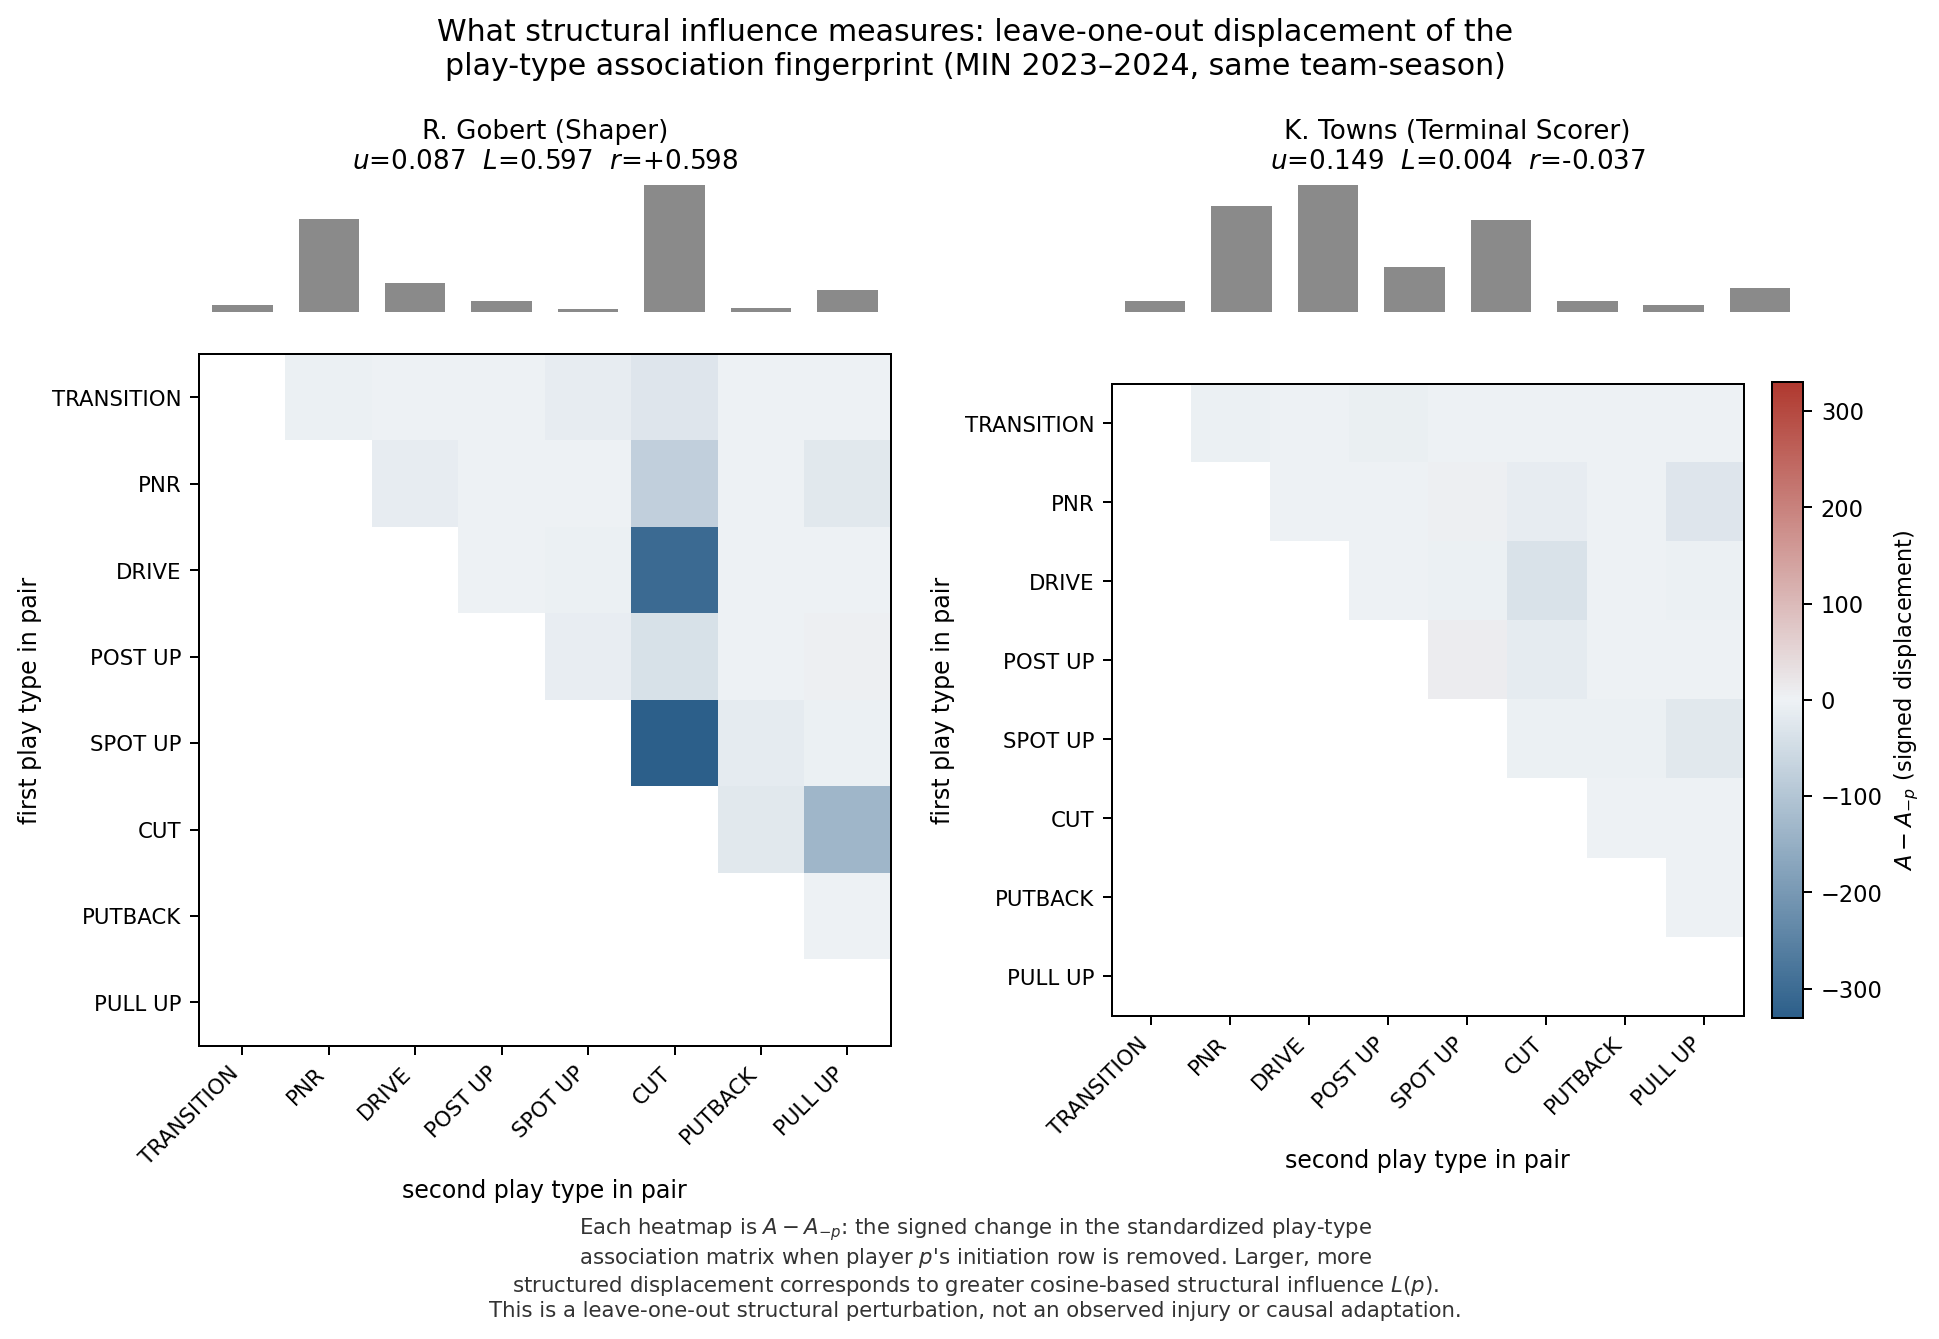
\includegraphics[width=\linewidth]{fig_loo_displacement.png}
\caption{\textbf{What structural influence measures: leave-one-out displacement of the play-type
association fingerprint.} Two players from the same team-season (Minnesota, 2023--24), same
$8\times 8$ play-type ordering, same diverging scale, diagonal blank. Each heatmap is
$\Afull-\Aminus{p}$, the signed change in the standardized play-type association matrix when
player $p$'s initiation row is removed; the bar strip above each panel is $p$'s own play-type
profile $\pt_p$, shown only for context. \emph{Left:} Rudy Gobert (\textsc{Shaper},
$u=0.09$, $\load=0.60$, $\resid=+0.60$): removing him collapses several \textsc{Cut}-linked
associations, a concentrated, deep displacement. \emph{Right:} Karl-Anthony Towns
(\textsc{Terminal Scorer}, $u=0.15$, $\load=0.00$, $\resid=-0.04$) on the same roster: removing
him leaves the fingerprint almost unchanged, a sparse, shallow displacement. The heatmap makes
structural influence visible as the \emph{pattern} (not merely the magnitude) of play-type
association links displaced by a player's removal. This is a leave-one-out structural
perturbation of the measured fingerprint, not an observed injury or causal adaptation.}
\label{fig:loo-displacement}
\end{figure}

\subsection{Usage-residual structural influence}
\label{sec:resid}

To guard against structural influence being a relabeling of usage, this paper regresses it on a quadratic in
usage $u$ across all classified players and retain the residual:
\begin{equation}
\label{eq:resid}
\load(p) \;=\; \beta_0+\beta_1 u_p+\beta_2 u_p^{2}+\resid(p),
\qquad
\resid(p) \;=\; \load(p)-\big(\hat\beta_0+\hat\beta_1 u_p+\hat\beta_2 u_p^{2}\big).
\end{equation}
Residual influence $\resid(p)$ is that same construct after removing the component predicted by
usage: structural influence that exceeds the level predicted by usage alone. Equivalently,
$\resid(p)$ is the organizational footprint that survives after accounting for involvement; this paper
shows it is stable within players and orthogonal to value. Here $u$ is the \emph{graph-native}
initiation share (a player's share of his team's initiations); the box-score
\emph{usage rate} reported in Table~\ref{tab:ortho} and used for the taxonomy median split is a
distinct, standard NBA measure. This paper residualizes on the graph quantity and reports correlations
against the box-score one, so the weak residual--usage correlations in Table~\ref{tab:ortho}
are not mechanical.

\subsection{The role taxonomy: making shapers visible}
\label{sec:taxonomy}

Crossing usage (consumption) with \emph{usage-residual} structural influence at a principled
cut discretizes the measurement into four labels. The vertical cut is the usage median
$u_{\text{med}}$ over the rotation pool (high vs.\ low volume). The horizontal cut is
$\resid(p)=0$: whether the player carries more structural influence than usage alone predicts
(Eq.~\ref{eq:resid}). Unequal class sizes are expected, most players sit at or below
expected influence, and are not a defect of the taxonomy.
\begin{equation}
\label{eq:taxonomy}
\text{role}(p)=
\begin{cases}
\textsc{Primary Organizer} & u_p\ge u_{\text{med}} \ \wedge\ \resid(p)> 0,\\[2pt]
\textsc{Shaper} & u_p< u_{\text{med}} \ \wedge\ \resid(p)> 0,\\[2pt]
\textsc{Terminal Scorer} & u_p\ge u_{\text{med}} \ \wedge\ \resid(p)\le 0,\\[2pt]
\textsc{Role Occupant / Specialist} & u_p< u_{\text{med}} \ \wedge\ \resid(p)\le 0.
\end{cases}
\end{equation}
Raw-influence median splits would force roughly equal quadrants and mislabel high-usage players
whose influence is only mechanically elevated by volume (negative residual). The residual cut
answers the question the construct asks: who displaces the wiring \emph{beyond} what usage
predicts? In basketball terms the two high-usage classes therefore split hubs through whom
initiation pathways are concentrically organized (\textsc{Primary Organizer}) from
high-volume creators/finishers whose influence is only what usage already predicts
(\textsc{Terminal Scorer}): including cases where both sit on the same roster
(Sec.~\ref{sec:emerge}). The taxonomy is a device for isolating the most visible
illustration of that construct (\textsc{Shaper}), not a four-class research
program. The other three labels are contrast strata. Scope for ``glue'' language is as in
Sec.~\ref{sec:intro}: offensive connective function in the initiation graph only. Robustness
to the usage threshold (45th/55th-percentile splits; residual cut fixed at zero) is in the
appendix.

% RECOMMENDED FIGURE (Figure 2): the 2D organizational-function map :  scatter of
%   every rotation player-season with x = usage, y = structural influence, quadrants
%   shaded, medians as crosshairs, ~12 labeled exemplars (Jokic/SGA organizers,
%   Gafford/Gobert hidden hubs, high-volume scorers as terminals).

\subsection{Displacement signature: the object of the portability test}
\label{sec:signature}

Structural influence is a scalar; portability requires the \emph{direction} of a player's footprint.
The \emph{adjacency-displacement signature} is the signed change in the fingerprint on removing
$p$:
\begin{equation}
\label{eq:signature}
\dA_p \;=\; \operatorname{vec}(\Afull)-\operatorname{vec}(\Aminus{p}) \;\in\;\mathbb{R}^{28}.
\end{equation}
$\dA_p$ records \emph{which} associations a player holds together. His \emph{play-type profile}
$\pt_p\in\Delta^{K-1}$ (his own normalized initiation distribution) is the \emph{table-visible}
description; $\dA_p$ is the \emph{graph-native} one. The portability test
(Section~\ref{sec:portability}) compares a player's cross-team $\dA_p$ similarity against that
of \emph{profile-matched decoys} (players with nearly identical $\pt$), so that any excess
similarity cannot be attributed to running the same plays.

% ---- notation table --------------------------------------------------------
\begin{table}[t]
\centering\small
\caption{Notation.}
\label{tab:notation}
\begin{tabular}{ll}
\toprule
Symbol & Meaning \\
\midrule
$\Bmat,\ \tilde{\Bmat}$ & player$\times$play-type initiation matrix; column-normalized form \\
$O$ & min-overlap co-initiation matrix, Eq.~\eqref{eq:overlap} \\
$\Amat=\Afull$ & fixed-margin standardized association matrix (fingerprint), Eq.~\eqref{eq:assoc} \\
$\Aminus{p}$ & association matrix with player $p$ removed \\
$\load(p)$ & structural influence = how much the offense's wiring depends on $p$, Eq.~\eqref{eq:load} \\
$\resid(p)$ & usage-residual structural influence, Eq.~\eqref{eq:resid} \\
$\dA_p\in\mathbb{R}^{28}$ & adjacency-displacement signature (player's structural footprint), Eq.~\eqref{eq:signature} \\
$\pt_p\in\Delta^{K-1}$ & player's play-type profile (table-visible) \\
$u_p$ & usage rate \\
\bottomrule
\end{tabular}
\end{table}

%=============================================================================
\section{A Confirmatory Program}
\label{sec:pipeline}

Contribution~A builds the instrument (Sec.~\ref{sec:framework}). Contribution~B asks what
it reveals, in the confirmatory order of Sec.~\ref{sec:intro} (restated as subsection
headers in Sec.~\ref{sec:results}). The analyses below are governed by the following
discipline.

\paragraph{Confirmatory discipline.}
The portability and efficiency analyses are \emph{pre-registered}. For each analysis the methods were fixed, before
touching outcome data: a single primary hypothesis and metric; a null model and inference
procedure; a \emph{feasibility gate} (a pre-committed check that the test is estimable, which
never inspects the primary effect); and binding \emph{stop conditions}, including a
\emph{no-fallback} clause forbidding post-hoc swaps of metric, outcome, or definition. Because
units are non-independent (players within team-seasons within franchises), inference uses
franchise- or team-season--clustered permutation and bootstrap procedures. This discipline is
what lets the efficiency null be read as an informative boundary rather than a failure to
re-run.

% RECOMMENDED FIGURE (Figure 3): vertical pipeline schematic :  Recoverability ->
%   Distinctness -> Behavior -> Efficiency boundary -> PORTABILITY (highlighted) ->
%   What predicts reproduction; annotate each with its one-line question.

%=============================================================================
\section{Results}
\label{sec:results}

Contribution~B, in order: does the measure reveal something new
(Sec.~\ref{sec:emerge}); is it just value (Sec.~\ref{sec:orthogonality}); does it match
observable basketball (Sec.~\ref{sec:behavior}); where does it stop
(Sec.~\ref{sec:efficiency}); does identity move when efficiency does not
(Sec.~\ref{sec:identity-resilience}, disclosed post-hoc); is it partly player-specific
(Sec.~\ref{sec:portability}); can transfer be predicted (Sec.~\ref{sec:travelfit}).

\subsection{Does the measure reveal something new?}
\label{sec:emerge}

Applying Eq.~\eqref{eq:taxonomy} to the rotation pool ($924$ player-seasons; the
pre-registered three-season sample, 2022--23 through 2024--25) yields four classes with
unequal size, as expected
under a residual cut (Table~\ref{tab:taxonomy}). The measurement separates players usage
cannot: \textsc{Shaper} players have structural influence ($0.078$) comparable to
\textsc{Primary Organizers} ($0.094$) while consuming far fewer possessions (usage $0.145$
vs.\ $0.244$), and scoring less than half as much ($9.0$ vs.\ $18.4$ ppg); their usage-residual
influence ($+0.062$) is the highest of any class. \textsc{Terminal Scorers} are the mirror
image, high usage ($0.233$), real scoring ($16.6$ ppg), near-zero residual influence ($-0.019$).
Most of the pool sits in the two non-excess-influence classes (terminal $40\%$, specialist $39\%$):
volume without excess structure, or neither.

The graph therefore identifies a type of
structural importance that conventional offensive volume measures do not see, organizer-level
displacement of the wiring at roughly half the scoring volume. This paper omits raw on-court net rating
from Table~\ref{tab:taxonomy}; whether that column would invite a value-premium reading is
tested in Sec.~\ref{sec:orthogonality}.

\begin{table}[t]
\centering\small
\caption{Organizational-function classes over the rotation pool ($n=924$ player-seasons,
2022-23 through 2024-25). Usage is box-score usage rate (distinct from the graph-native
initiation share $u$ in Eq.~\ref{eq:resid}). Influence is $\load(p)$ (Eq.~\ref{eq:load}); residual influence is $\resid(p)$ (Eq.~\ref{eq:resid}). Classes use usage median $\times$ $\resid>0$
(Eq.~\ref{eq:taxonomy}), not equal-mass raw-influence medians. Raw on-court net rating is omitted
from this table and examined as a falsification test in Sec.~\ref{sec:orthogonality}. The
\textsc{Shaper} row is the most visible illustration of the construct; other rows are
contrast.}
\label{tab:taxonomy}
\begin{tabular}{lrrrrrrr}
\toprule
Class & $n$ & \% pool & Usage & Influence & Resid.\ influence & PPG & MPG \\
\midrule
\textsc{Primary Organizer} & 96 & 10.4 & 0.244 & 0.094 & $+0.054$ & 18.4 & 29.6 \\
\textsc{Shaper} & 103 & 11.1 & 0.145 & 0.078 & $+0.062$ & 9.0 & 23.6 \\
\textsc{Terminal Scorer} & 368 & 39.8 & 0.233 & 0.014 & $-0.019$ & 16.6 & 28.6 \\
\textsc{Role Occupant / Special.} & 357 & 38.6 & 0.147 & 0.006 & $-0.009$ & 8.2 & 22.8 \\
\bottomrule
\end{tabular}
\end{table}

Table~\ref{tab:exemplars} and Figure~\ref{fig:taxonomy-map} put the same names on that
axis. The Organizer/Terminal split is not ``who creates'' versus ``who scores'', both
classes take high usage and initiate a lot. It asks a more specific on-court question:
\emph{when this player leaves the floor, does the team's map of who starts which play
types reorganize beyond what losing that much volume would imply?}

\paragraph{How structural classes differ in offensive initiation.}
The graph does not track assists, within-possession passing chains, screens set without
initiation credit, gravity, or communication. An \emph{initiator} is as defined in
Sec.~\ref{sec:data}. Class-average initiation diets make the
roles concrete.
\textsc{Primary Organizers} start half-court offense on the ball: pick-and-roll
($\approx\!24\%$), drives ($\approx\!19\%$), and post-ups ($\approx\!16\%$) lead their mix.
\textsc{Terminal Scorers} look similar at first glance, drives and pick-and-rolls also
dominate, but carry more spot-up volume and, critically, less unique overlap across those
jobs: other players already start the same combinations, so removing the star mostly
subtracts possessions rather than rewriting who-holds-which-jobs.
\textsc{Shaper} players are not primary handlers. Their diet is cut-and-roll
interior work: pick-and-roll ($\approx\!25\%$) and cuts ($\approx\!23\%$) together nearly
half their initiations, rim runs, dive cuts, and roll starts that occupy initiation roles
overlapping across ball-screen and off-ball actions. \textsc{Role Occupants} are mostly
spot-up specialists ($\approx\!33\%$ spot-ups). High $\resid$ means the player's initiation
jobs are \emph{shared across play types} in a way the rest of the rotation does not
duplicate; it is organizational dependence, not a second box-score of ``hustle.''

\paragraph{Named contrast.}
Same seasons bolded in Table~\ref{tab:exemplars} and labeled in
Figure~\ref{fig:taxonomy-map}. On 2023--24 Oklahoma City, SGA is the on-ball hub: drives
$\approx\!34\%$, pull-ups $\approx\!24\%$, pick-and-rolls $\approx\!18\%$ of his
initiations, and he alone starts roughly a third of Thunder drives and pull-ups and nearly
half their post-ups ($\resid=+0.22$). Denver 2024--25 is the same shape with Joki\'c as the
half-court hub (pick-and-roll and post-up lead his diet; he starts over half of Denver's
post-ups; $\resid=+0.067$). By contrast, 2023--24 Los Angeles has \emph{two} high-usage
stars in opposite classes: the dotted link in Figure~\ref{fig:taxonomy-map}. LeBron
(drives and pick-and-rolls at star volume; $\resid=-0.054$) is a Terminal Scorer: the
coaching ``point forward'' label fits what he does with the ball, but those initiation jobs
are ones the roster can redistribute. Anthony Davis (pick-and-roll, post-up, and cuts;
$\approx\!42\%$ of Lakers post-up starts and $\approx\!31\%$ of their cuts;
$\resid=+0.105$) is the Organizer: the interior/ball-screen hub next to LeBron's volume.
Boston 2022--23 is the wing version of the same split, Tatum's drive/pick-and-roll/spot-up
volume with $\resid\le 0$, while the motion offense keeps those starts shared.

So ``point forward'' and ``primary creator'' name on-ball skill. $\resid$ asks whether the
offense's starting jobs are concentrically organized through that player. SGA's Thunder and
Joki\'c's Nuggets are; that Lakers season is organized through Davis's post/cut/pick-and-roll
overlap even while LeBron dominates usage; Tatum's Celtics are organized through the system.

The sharpest illustration is the low-usage half of the same split. Gobert and Gafford are
not traditionally described as offensive organizers: they do not create for teammates in
the box-score sense. Yet they carry organizer-level structural dependence without the
volume. Gobert alone started $\approx\!62\%$ of Minnesota's cuts in 2023--24 (cut and
pick-and-roll $\approx\!74\%$ of his own initiations), not a creator, but a node the
offense's geometry depends on. That is what usage cannot see, and why shapers are the
class the instrument was built to make visible. Hart is a Role Occupant: mixed
spot-up / pick-and-roll / drive volume that others cover. Secondary table rows are
additional in-class examples not labeled on the figure.

\begin{figure}[H]
 \centering
 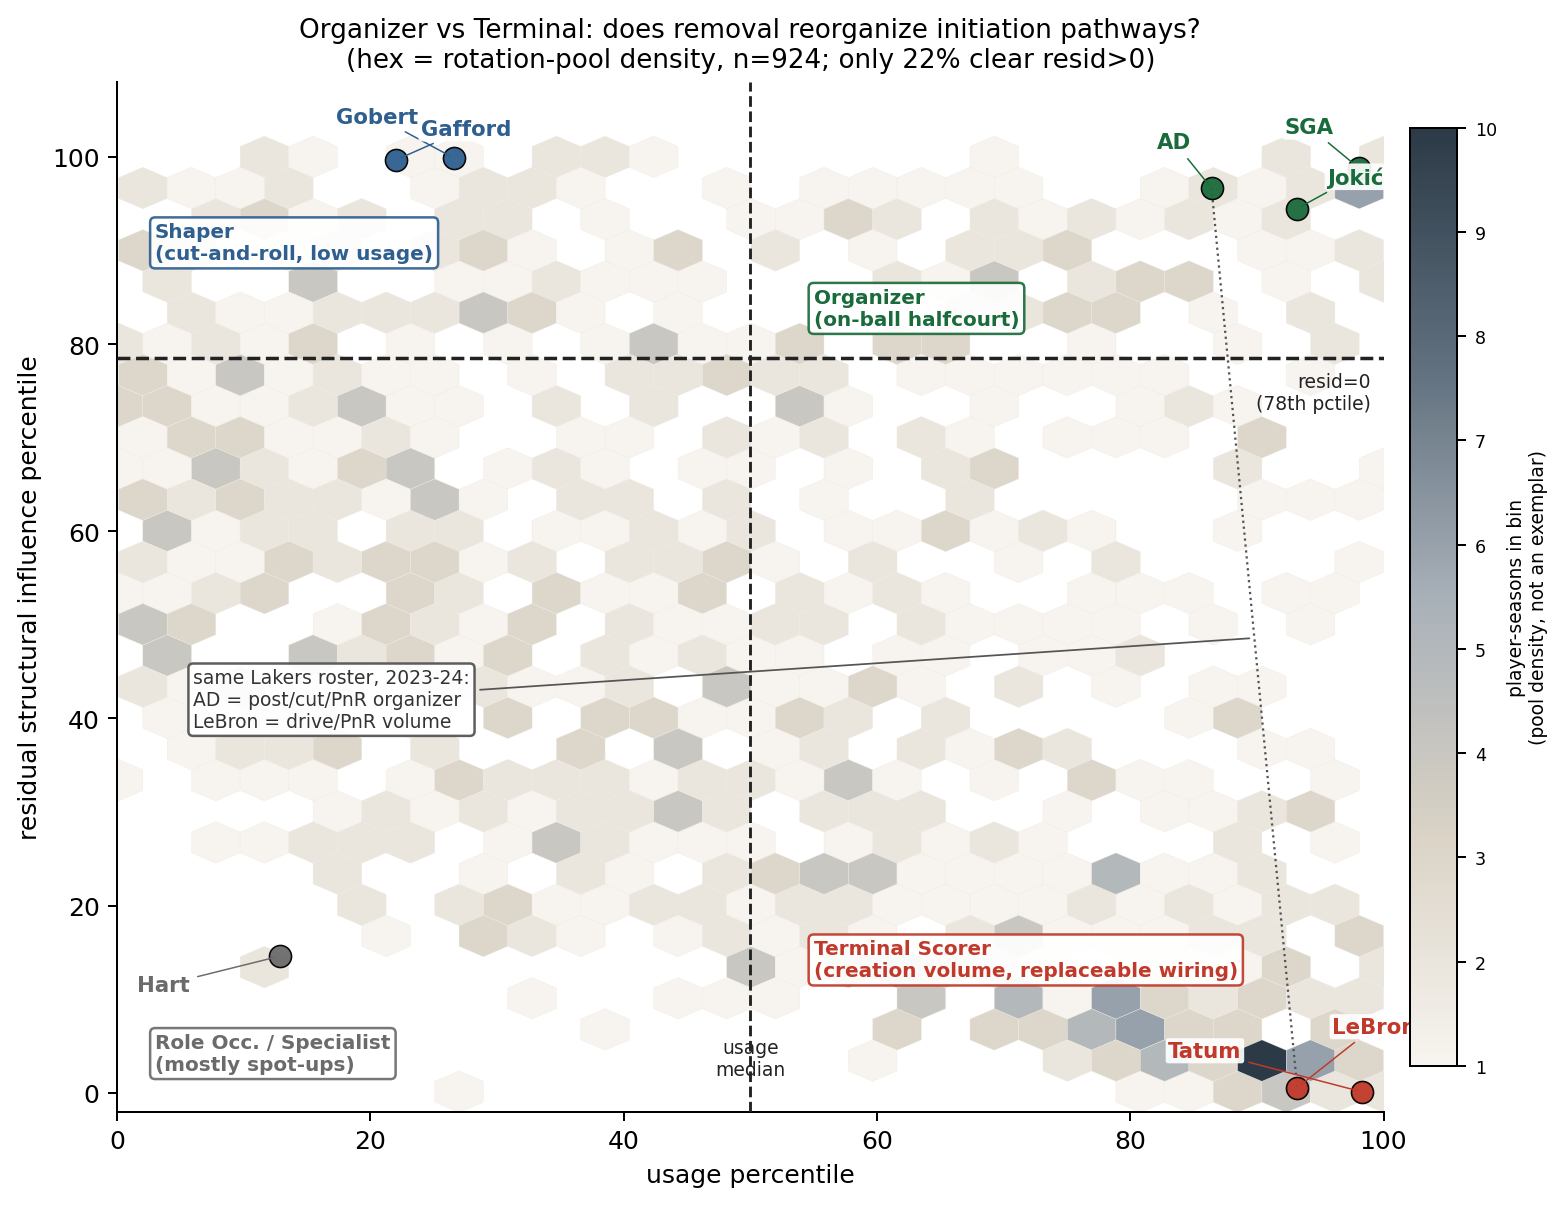
\includegraphics[width=0.92\textwidth]{fig_taxonomy_map.png}
 \caption{\textbf{Organizer vs.\ Terminal on one map.} Both axes are percentile ranks of
 the rotation pool ($n=924$). Vertical dashed line: usage median. Horizontal dashed line:
 $\resid=0$ (Eq.~\ref{eq:taxonomy}), at the $\approx\!78$th residual percentile, only
 $\approx\!22\%$ of the pool clears it. Bold rows in Table~\ref{tab:exemplars} are the
 labeled points. In basketball terms: SGA/Joki\'c/AD are high-usage half-court initiation
 hubs (pick-and-roll / post / drive overlap, $\resid>0$); Gobert/Gafford are low-usage
 cut-and-roll hubs; LeBron/Tatum take star creation volume with $\resid\le 0$; Hart is a
 replaceable Role Occupant. The dotted link is the within-roster illustration: on the
 2023--24 Lakers, Davis holds the post/cut/pick-and-roll overlap while LeBron holds
 high-usage volume. Hexbin shading is pool density only (dark bin near Tatum $=$ many
 Terminals, not one player).}
 \label{fig:taxonomy-map}
\end{figure}

\begin{table}[t]
\centering\small
\caption{Named exemplars of the taxonomy (one player-season each). Usage is box-score usage
rate and influence is $\load(p)$, as in Table~\ref{tab:taxonomy}; residual influence is usage-adjusted
$\resid(p)$. Bold-season rows are the points labeled in Fig.~\ref{fig:taxonomy-map} (the
Organizer/Terminal/Shaper story in the text). Remaining rows are additional in-class
examples. All organizers and shapers have $\resid>0$; terminals and specialists have
$\resid\le 0$. The Lakers 2023--24 pair (Davis Organizer, James Terminal) is the
within-roster contrast. Gafford's primary row is his full WAS 2022--23 season, not the
partial pre-trade WAS 2023--24 stint in Table~\ref{tab:cases}. Illustrations, not a ranking.}
\label{tab:exemplars}
\begin{tabular}{lllcrrr}
\toprule
Class & Player & Team & Season & Usage & Influence & Resid.\ influence \\
\midrule
\textsc{Organizer}
 & \textbf{S.\ Gilgeous-Alexander} & \textbf{OKC} & \textbf{2023--24} & \textbf{0.317} & \textbf{0.308} & $\mathbf{+0.216}$ \\
 & \textbf{A.\ Davis} & \textbf{LAL} & \textbf{2023--24} & \textbf{0.261} & \textbf{0.168} & $\mathbf{+0.105}$ \\
 & \textbf{N.\ Joki\'c} & \textbf{DEN} & \textbf{2024--25} & \textbf{0.285} & \textbf{0.145} & $\mathbf{+0.067}$ \\
 & B.\ Adebayo & MIA & 2023--24 & 0.247 & 0.211 & $+0.166$ \\
 & D.\ Ayton & POR & 2023--24 & 0.211 & 0.327 & $+0.305$ \\
 & A.\ Sengun & HOU & 2023--24 & 0.270 & 0.136 & $+0.093$ \\
\midrule
\textsc{Shaper}
 & \textbf{R.\ Gobert} & \textbf{MIN} & \textbf{2023--24} & \textbf{0.152} & \textbf{0.620} & $\mathbf{+0.598}$ \\
 & \textbf{D.\ Gafford} & \textbf{WAS} & \textbf{2022--23} & \textbf{0.146} & \textbf{0.411} & $\mathbf{+0.397}$ \\
 & J.\ Poeltl & TOR & 2023--24 & 0.160 & 0.217 & $+0.203$ \\
 & J.\ Allen & CLE & 2024--25 & 0.156 & 0.110 & $+0.088$ \\
 & W.\ Kessler & UTA & 2023--24 & 0.127 & 0.239 & $+0.227$ \\
 & J.\ Duren & DET & 2022--23 & 0.139 & 0.240 & $+0.227$ \\
\midrule
\textsc{Terminal Scorer}
 & \textbf{L.\ James} & \textbf{LAL} & \textbf{2023--24} & \textbf{0.285} & \textbf{0.013} & $\mathbf{-0.054}$ \\
 & \textbf{J.\ Tatum} & \textbf{BOS} & \textbf{2022--23} & \textbf{0.319} & \textbf{0.009} & $\mathbf{-0.090}$ \\
 & J.\ Brown & BOS & 2022--23 & 0.307 & 0.023 & $-0.050$ \\
 & F.\ Wagner & ORL & 2023--24 & 0.250 & 0.011 & $-0.044$ \\
 & C.\ McCollum & NOP & 2022--23 & 0.260 & 0.035 & $-0.027$ \\
\midrule
\textsc{Role Occupant / Specialist}
 & \textbf{J.\ Hart} & \textbf{NYK} & \textbf{2023--24} & \textbf{0.133} & \textbf{0.003} & $\mathbf{-0.022}$ \\
 & M.\ Smart & BOS & 2022--23 & 0.176 & 0.001 & $-0.020$ \\
 & D.\ Finney-Smith & BKN & 2022--23 & 0.129 & 0.005 & $-0.007$ \\
 & O.\ Anunoby & NYK & 2023--24 & 0.173 & 0.001 & $-0.011$ \\
 & J.\ Holiday & BOS & 2024--25 & 0.156 & 0.001 & $-0.017$ \\
\bottomrule
\end{tabular}
\end{table}

\subsection{Is it just another value metric?}
\label{sec:orthogonality}

If structural influence merely relabeled usage, scoring, or net rating, the measurement would be
uninteresting. This paper treats on-court net rating as a falsification test of that hidden-premium
hypothesis (Sec.~\ref{sec:intro}): either an apparent shaper edge that team quality
explains away, or no apparent edge at all, would falsify a hidden shaper value premium.

Under the residual cut, organizers already lead shapers on raw on-court net rating
($+1.45$ vs.\ $+0.80$), so there is no apparent ``shaper premium'' to begin with. Once net
rating is residualized within team-season, the organizer median remains above the shaper
median ($+1.22$ vs.\ $+0.50$) but the gap does not clear conventional significance
(Mann--Whitney $p=0.10$, two-sided). Spearman correlations over $n=1{,}283$ player-seasons
(Table~\ref{tab:ortho}) confirm the separation: usage-residual influence is essentially
\emph{uncorrelated with net rating}, $\rho(\resid,\text{net rating})=-0.018$. Raw influence
correlates only modestly with volume (points $\rho=0.44$, touches $\rho=0.38$); residual
ties to volume are weak and negative ($|\rho|\le0.26$). As shown here, organizational
function is a separable axis from conventional value.

\begin{table}[t]
\centering\small
\caption{Distinctness of organizational function from traditional metrics (Spearman $\rho$,
$n=1{,}283$ player-seasons with complete box-score coverage, broader than the $924$-season
rotation pool in Table~\ref{tab:taxonomy}). The key cell is
$\rho(\resid,\text{net rating})=-0.018$: organizational function is orthogonal to value.}
\label{tab:ortho}
\begin{tabular}{lrr}
\toprule
Metric & $\rho(\load,\cdot)$ & $\rho(\resid,\cdot)$ \\
\midrule
Usage rate & $+0.270$ & $-0.261$ \\
Points per game & $+0.436$ & $-0.264$ \\
Assists per game & $+0.278$ & $-0.255$ \\
Assist \% & $+0.106$ & $-0.190$ \\
Touches & $+0.376$ & $-0.253$ \\
Frontcourt touches & $+0.424$ & $-0.238$ \\
\textbf{Net rating (value)} & $+0.203$ & $\bm{-0.018}$ \\
\bottomrule
\end{tabular}
\end{table}

\subsection{Does it correspond to observable basketball?}
\label{sec:behavior}

Having measured who the wiring depends on, and shown that dependence is not a value premium
(Sec.~\ref{sec:orthogonality}), this paper checks whether the class corresponds to recognizable
offensive behavior: the class-level version of the rim-running, cut-and-roll interior role
illustrated by shaper exemplars in Table~\ref{tab:exemplars}, not a biography of any one
player. Using within-team-season comparisons on the on-court subset, this paper asks whether shaper
presence is associated with changes in play-type mix. This corroborates that the structural
class is visible on the floor.

\paragraph{Shaper presence and play mix.}
Across $73$ team-seasons with both strata, shaper presence shifts the mix toward off-ball
and ball-screen actions and away from spot-up and drive actions: cuts $+1.35$ pp,
pick-and-roll $+0.98$ pp; spot-ups $-1.25$ pp, drives $-0.54$ pp
(percentage points of share, within-team). The low-usage character of the class makes the
interpretation especially clean: a mix shift when shapers are on the floor is less
mechanically attributable to the shaper simply taking more of his own shots, and more
readily read as reorganization among other players. Primary organizers reshape the mix even
more sharply (post-ups $+2.33$ pp, pick-and-roll $+0.96$ pp; $58$ team-seasons), useful
contrast, not a second subject. The team-season count differs between strata ($73$ vs.\
$58$) because a team-season only enters this comparison if it has at least one on-court
possession with the stratum present and at least one without; which team-seasons clear that bar
depends on the class, since organizer and shaper presence are not perfectly co-located across
rosters. The observed play-type mix shifts with shaper presence.

Two caveats bound these as \emph{associations}, not causal estimates: high-usage classes
mechanically run more of their own play types when present (which is why the shaper
contrast is especially informative), and a class being off the floor overlaps with bench and
garbage-time lineups, within-team-season differencing removes team identity but not game
state.

\paragraph{A refinement: re-channeling, not expanding, the repertoire.}
Shaper presence appears to re-channel an offense's existing repertoire rather than expand
it: it redistributes which initiating-role-to-play-type routes occur without increasing route
entropy or reducing route concentration. Modeling each possession's initiating-role$\to$
play-type route, this paper finds no increase in route entropy or reduction in concentration for other
roles under shaper presence. The intuitive alternative, that more shapers create
\emph{more} distinct pathways, is not supported. Shaper presence is associated with
\emph{which} actions the offense runs within a repertoire bounded by the personnel on the
floor, not with a wider menu.

% RECOMMENDED FIGURE (Figure 6): (a) diverging bar chart of shaper within-team
%   play-mix deltas; (b) route-entropy shaper-present vs absent (near-zero delta),
%   captioned "reshapes, does not broaden."

\subsection{Where does the construct stop?}
\label{sec:efficiency}

The instrument measures organization, not scoring. A natural first question about any new
construct is whether it independently predicts the outcome everyone already optimizes: here,
offensive points per possession. This paper pre-registers the tempting claim that a structurally
\emph{complete} offense (creation, connection, and conversion all present) scores more
efficiently, with a frozen talent control and a binding no-fallback clause. It does not
hold. A measurement of organizational structure need not reproduce the outcomes used to
evaluate players. The null therefore defines the construct's boundary: structural
dependence is measurable, but it is not equivalent to offensive efficiency.

\paragraph{Design.}
On the on-court subset (all five players classified; $N=4.2\times10^{5}$, $90$ team-seasons),
define coverage
\begin{equation}
\label{eq:covered}
\textsc{Covered}_i \;=\; \mathbb{1}\big[\,n^{\text{org}}_i\ge 1 \ \wedge\
n^{\text{shap}}_i\ge 1 \ \wedge\ n^{\text{term}}_i\ge 1\,\big],
\end{equation}
and estimate
\begin{equation}
\label{eq:coverage}
\PPP_i = \beta\,\textsc{Covered}_i
 + \textstyle\sum_{c} a_c\, n^{c}_i
 + g\,\text{Talent}_i
 + \phi_{\text{ts}(i)} + \psi_{\text{opp}(i)} + \chi_{\text{per}(i)} + \omega_{\text{sb}(i)}
 + \varepsilon_i .
\end{equation}
The linear role counts are included, so, because $\textsc{Covered}$ is a nonlinear threshold of
them, $\beta$ isolates \emph{completeness} beyond having more of each role. $\text{Talent}_i$
is a frozen control (mean over the five of each player's leave-current-game-out
points-per-initiation); fixed effects absorb team-season, opponent, period, and score-margin;
inference clusters by team-season.

\begin{hypothesis}[Coverage $>$ accumulation, T$_{\text{cov}}$]
\label{hyp:cov}
$\beta>0$ with team-season cluster-robust $p<0.01$ and a cluster-bootstrap $95\%$ CI excluding
$0$.
\end{hypothesis}

\paragraph{Result: the boundary.}
The gate passed cleanly, coverage varies within teams and remains near-orthogonal to the talent
index by construction, so the test had genuine room to detect an effect. It did not:
$\hat\beta=+0.42$ points per $100$ possessions ($t=0.53$, $p=0.60$), team-season
cluster-bootstrap $95\%$ CI $[-1.15,+1.90]$ straddling zero, with the play-type-FE and
talent-removed specifications agreeing closely (Table~\ref{tab:coverage}). The one robust
driver is accumulation of \emph{organizers} ($+2.35$ per $100$, $t=4.62$). \emph{Structural
completeness does not improve efficiency beyond talent at any detectable level.} Precision
here is set by the $90$ team-season clusters, not the $4.2\times10^{5}$ possessions: the
cluster-robust standard error is $\approx0.78$ points per $100$, giving a minimum detectable
effect at $80\%$ power of $\approx2.2$ points per $100$. This paper can therefore rule out a
\emph{large} completeness bonus but not a modest one, the CI's upper bound ($+1.90$) is not
zero. Because coverage is provably separable from talent (so the test had room to detect an
effect), and the estimate is small and stable across specifications, this paper reads this as a
credible \emph{boundary at the pre-registered bar}, not proof of an exact null.

\begin{table}[t]
\centering\small
\caption{Efficiency boundary (possession-level PPP, $N\!=\!4.2\times10^{5}$, $90$ team-seasons).
Coefficients in points per $100$; CIs team-season cluster-bootstrap. $\textsc{Covered}$ is never
distinguishable from zero; organizer accumulation is the robust driver.}
\label{tab:coverage}
\begin{tabular}{lrrl}
\toprule
Specification / term & pts/100 & $t$ & 95\% CI \\
\midrule
\textsc{Covered}: primary (M1) & $+0.42$ & $0.53$ & $[-1.15,+1.90]$ \\
\textsc{Covered}: with play-type FE & $+0.44$ & $0.53$ & $[-1.29,+2.04]$ \\
\textsc{Covered}: talent control removed & $+0.43$ & $0.54$ & $[-1.15,+1.94]$ \\
\textsc{Covered}: $\ge 4/5$ classified & $+0.26$ & $0.37$ & $[-1.23,+1.67]$ \\
\midrule
$n_{\text{organizer}}$ (accumulation) & $+2.35$ & $4.62$ & -- \\
\bottomrule
\end{tabular}
\end{table}

\paragraph{Reading the boundary.}
Organizational function describes how an offense is \emph{wired}; whether the resulting
actions become points is governed by the talent executing them
(Sec.~\ref{sec:orthogonality}). One registered caveat: the talent control under-measures
shapers by construction, but the talent-removed specification gives a materially identical
estimate ($+0.43$ vs.\ $+0.42$), so measured talent is not masking a completeness effect. The
licensed reading is the boundary itself: conditional on measured talent, structural
completeness is not an independent PPP premium. That is a finding about what the construct
is \emph{not}, and it leaves intact what the instrument enables: studying organization as
its own object.

\paragraph{Isolating shaper presence alone.}
\textsc{Covered} tests whether having the three structural functions on the floor
(organizer, shaper, and terminal; Eq.~\ref{eq:covered}) buys points. The fourth taxonomy
class, \textsc{Role Occupant / Specialist}, is not required for completeness: low usage and
low influence means it does not fill a creation, connection, or conversion job. A narrower, more
direct version of the practitioner's question is whether merely having a
shaper present, regardless of completeness, changes scoring. This paper reran the identical
team-season-demeaned design with $\textsc{Covered}$ replaced by
$\text{HasShaper}_i=\mathbb{1}[n^{\text{shap}}_i\ge1]$, retaining the linear role counts so the
coefficient is shaper presence net of accumulation. On the same $N=4.2\times10^{5}$
possessions, the raw within-team-season gap (shaper on floor minus off, no other controls)
is $+0.25$ points per $100$; with the full control set,
$\widehat{\text{HasShaper}}=+0.00$ points per $100$ ($t=0.00$, $p=1.00$), team-season
cluster-bootstrap $95\%$ CI $[-1.37,+1.48]$. The linear $n_{\text{shaper}}$ accumulation
term is nominally different from zero at conventional significance ($+1.17$ per $100$,
$t=2.25$, $p\approx0.02$) but does not clear the pre-registered $p<0.01$ confirmatory bar, so this paper
does not treat it as a confirmed accumulation effect; it is smaller and less robust than organizer
accumulation, which is robust in every specification in this section, and this paper does not re-estimate
it here and refer to Table~\ref{tab:coverage}'s single frozen figure ($+2.35$, $t=4.62$).
Whether the question is completeness or shaper presence
alone, the answer is the same null: shapers reorganize what an offense runs
(Sec.~\ref{sec:behavior}) without moving offensive points per possession.
These tests are \emph{offensive} PPP (points scored while the shaper is on the floor for
his team's possessions). A two-way on-court net rating (offense plus defense with the same
five) is a separate diagnostic; the possession graph does carry defensive on-court lineups,
but that test is not part of the pre-registered efficiency boundary reported here. Across
$90$ team-seasons with team-season fixed effects and an offense-only design, shaper
presence, whether measured as completeness or in isolation, is not distinguishable from a
null effect on offensive PPP.

\subsubsection{Exploratory: does the HasShaper null hide tier heterogeneity?}
\label{sec:shaper-tiers}
As a post-hoc check (motivated by an out-of-sample 2025--26 review; Sec.~\ref{sec:data}),
this paper splits \textsc{Shaper} at within-class median residual influence into hub vs.\
marginal, then split marginal by position (big vs.\ wing). Replacing $\textsc{Covered}$
with three presence indicators on the same pre-registered three-season sample yields
Table~\ref{tab:shaper-tiers}: \emph{none} of the three tiers clears the paper's $0.01$
confirmatory bar. The check is exploratory relative to the pre-registered efficiency
tests and does not revise Table~\ref{tab:coverage} or the \textsc{HasShaper} null above.

\begin{table}[h!]
\centering\small
\caption{Exploratory shaper-tier PPP effects ($N\!=\!420{,}993$, $90$ team-seasons).
Coefficients in points per $100$; confirmatory bar $p<0.01$ as reporting benchmark only.}
\label{tab:shaper-tiers}
\begin{tabular}{lrrl}
\toprule
Tier & pts/100 & $p$ & Confirmatory bar ($p<0.01$) \\
\midrule
HasHub & $+1.10$ & $0.077$ & not met \\
HasMargBig & $+1.70$ & $0.025$ & not met \\
HasMargWing & $+1.29$ & $0.122$ & not met \\
\bottomrule
\end{tabular}
\end{table}

\subsubsection{Exploratory: identity moves when efficiency does not}
\label{sec:identity-resilience}

The efficiency boundary answers what structural dependence is \emph{not}: it is not an
independent PPP premium. The natural construct-native follow-up is whether dependence is
still visible in \emph{offensive identity} under real substitution: the association
fingerprint of who jointly holds which play-type jobs, even when points per possession do
not move. That is the question this subsection answers. It was \emph{not}
pre-registered. Like the tier split above, it is a disclosed post-hoc test motivated by
the boundary finding itself: if organization is measurable but not equivalent to scoring,
the licensed ``so what'' must be organizational. This paper therefore tests identity displacement,
not a second scoring screen, and does not treat the result as part of the original
confirmatory protocol.

\paragraph{Not the same quantity as $\load(p)$.}
Structural influence (Eq.~\ref{eq:load}) is a \emph{season-level leave-one-out counterfactual}:
delete player $p$'s initiation row from $\Bmat$, recompute $\Amat$, and measure cosine
displacement of the full-season fingerprint. The taxonomy that labels
\textsc{Shaper} versus \textsc{Role Occupant / Specialist} is built from
usage-residual $\resid(p)$ of that same leave-one-out $\load(p)$. Comparing class means
on $\load(p)$ itself would largely re-derive the classification. The outcome here is
different. For each rotation player-season with adequate sample ($\ge 400$ possessions on
and $\ge 400$ off), this paper splits the team's actual possessions by whether $p$ was
\emph{on the floor}, build standardized association matrices $\Amat_{\mathrm{on}}$ and
$\Amat_{\mathrm{off}}$ from those observed subsets, and define the on/off identity
displacement
\begin{equation}
\label{eq:DA}
D_A(p) \;=\; 1-\cossim\!\big(\operatorname{vec}(\Amat_{\mathrm{on}}),\,
\operatorname{vec}(\Amat_{\mathrm{off}})\big).
\end{equation}
$D_A$ is ecological: it uses real benchings and rest patterns, not a hypothetical
full-season removal. A secondary mix measure $D_\pi$ is the total-variation distance
between on-court and off-court play-type share vectors. Theory predicts that leave-one-out
$\load(p)$ and on/off $D_A(p)$ should be related: both ask how much the fingerprint moves
when $p$ is absent, but they are not algebraically the same object. The test's force is
whether the season-level counterfactual shows up under observed substitution.

\paragraph{Design.}
Among $908$ rotation player-seasons meeting the on/off sample gate, this paper compares class means
of $D_A$, then (as the licensed contrast) match each \textsc{Shaper} to a
\textsc{Role Occupant / Specialist} nearest neighbor on usage (caliper $0.03$ usage
points; prefer same team-season; no replacement). \textsc{Primary Organizer} is reported
only as a high-usage positive-control reference and is not part of the matched claim.
Terminal scorers are a secondary matched contrast (fewer pairs within caliper). This paper also
reports $\operatorname{corr}(\load,D_A)$ after residualizing both sides on $\log\min(n_{\mathrm{on}},n_{\mathrm{off}})$
and usage, as a continuous construct check.

\paragraph{Result.}
Unmatched means already separate the taxonomy along identity, not only along the
leave-one-out influence used to build it (Table~\ref{tab:identity-resilience}): organizers and
shapers show roughly twice the on/off fingerprint displacement of terminals and role
occupants. The primary matched test is decisive: among $96$ shaper--role-occupant pairs
(mean usage gap $0.008$; $81$ within the same team-season), mean paired
$\Delta D_A=+0.115$ ($t=6.35$, $p\approx 7\times 10^{-9}$), with the shaper larger in
$81\%$ of pairs. Play-type mix also shifts more under shaper absence
(paired $\Delta D_\pi=+0.011$, $t=4.06$, $p\approx 10^{-4}$). The thinner
shaper--terminal match ($n=25$) agrees in sign for $D_A$
($\Delta=+0.078$, $p\approx 0.026$). Continuously, leave-one-out $\load(p)$ predicts
on/off $D_A$ after minute and usage controls ($r=+0.60$, $n=908$), including within
shapers alone ($r=+0.79$), ecological validity for the season-level construct, not a
restatement of Eq.~\ref{eq:load}.

\begin{table}[h!]
\centering\small
\caption{On/off offensive-identity displacement $D_A$ (Eq.~\ref{eq:DA}) by structural class.
Not pre-registered. $N=908$ rotation player-seasons with $\ge 400$ possessions on and off.
Organizers are a reference class; the licensed claim is the usage-matched
shaper vs.\ role-occupant contrast in the text ($\Delta D_A=+0.115$, $n=96$ pairs).}
\label{tab:identity-resilience}
\begin{tabular}{lrrrr}
\toprule
Class & $n$ & mean $D_A$ & median $D_A$ & mean usage \\
\midrule
Primary Organizer & 96 & $0.214$ & $0.170$ & $0.244$ \\
Shaper & 102 & $0.202$ & $0.151$ & $0.144$ \\
Terminal Scorer & 361 & $0.112$ & $0.094$ & $0.233$ \\
Role Occupant / Specialist & 349 & $0.102$ & $0.085$ & $0.148$ \\
\bottomrule
\end{tabular}
\end{table}

\paragraph{Licensed reading.}
Efficiency does not move with shaper presence (Sec.~\ref{sec:efficiency}); offensive
\emph{identity} does, under real substitution, relative to usage-matched non-organizers.
The construct-native value of the shaper class, on this evidence, is contribution to
maintaining the team's measured association fingerprint when that player is on the floor, not
a PPP or dollar premium. Because the test is post-hoc, this paper reports it as a disclosed
follow-up that answers the boundary, not as a pre-registered confirmation. A prospective
replication on a held-out season remains the gold-standard check.

\subsection{Is organizational function partly player-specific?}
\label{sec:portability}

The portability analysis is a supporting construct-validity check (does a player-associated
component of measured organizational function reappear after a team change?), not the paper's
primary claim. Having established that the construct is visible on the floor
(Secs.~\ref{sec:behavior}--\ref{sec:efficiency}) and bounded for efficiency, this paper turns to that
transfer question. If a player's high structural influence reflects something about the player
rather than only the old team around him, his measured wiring footprint should
reappear after he changes teams. This paper answers with a pre-registered portability test on all
movers, then examine the shaper subclass as a measurement stress test: the class where
low usage most clearly hides structural dependence.

\paragraph{Design.}
For a player $p$ with two chronologically adjacent franchise stints, let
$\dA_p^{\text{orig}},\dA_p^{\text{dest}}$ be his displacement signatures
(Eq.~\ref{eq:signature}) and
$\text{self\_sim}(p)=\cossim(\dA_p^{\text{orig}},\dA_p^{\text{dest}})$. Movers are pairs of
the player's own consecutive included stints, ordered by first-game date (\texttt{anchor}), with the
earlier stint labeled origin and the later destination. The threat to identification is that a
portable signature could merely reflect a portable \emph{play-type profile} (``he runs the same
plays everywhere''). This paper neutralizes it with \emph{profile-matched decoys}: for each mover the procedure takes
$K=5$ destination-team players whose profile $\pt$ is closest to $p$'s and compute
$\text{decoy\_sim}(p)$, the similarity of $p$'s origin signature to those decoys' destination
signatures. The portability statistic is the per-player excess
\begin{equation}
\label{eq:portability}
\Delta(p) \;=\; \text{self\_sim}(p)-\text{decoy\_sim}(p),
\end{equation}
so that a positive $\Delta$ means the player's own structural footprint predicts his
destination footprint better than that of a teammate who runs the same plays.

\begin{hypothesis}[Portability, T1]
\label{hyp:port}
$\operatorname{median}_p \Delta(p)>0$, with a matched-set (within-pool) exchangeability
permutation $p<0.01$ and a destination-franchise cluster-bootstrap $95\%$ CI excluding $0$.
\end{hypothesis}

\paragraph{Feasibility and identification.}
The gate confirmed $294$ movers in the pre-registered three-season window
(2022--23 through 2024--25)
across $30$ destination franchises, each with $\ge3$
profile-matched decoys, and, critically, that the signature is \emph{not} a restatement of
the profile: the absolute Spearman correlation between profile cosine and signature cosine is
only $0.007$. Displacement signatures are essentially uncorrelated with play-type profiles,
so a positive $\Delta$ cannot be dismissed as ``he runs the same plays.'' Movers are
identified by NBA person ID and required to be \emph{truly} chronologically adjacent, ordered
by each stint's first game date rather than by season label alone: two different team-stints
can carry the same season label after a mid-season trade, and ordering by label alone breaks
that tie arbitrarily rather than chronologically, silently mis-pairing the wrong two stints
across a season boundary.

\paragraph{Result: a player-specific component persists on average.}
On the same pre-registered mover sample ($n=294$), median
self-similarity is $+0.129$ versus median decoy similarity
$+0.049$, a median excess $\Delta=+0.056$. All three pre-registered criteria pass: $\Delta>0$;
a matched-set exchangeability permutation (each mover's $\{\text{self}\}\cup\{\text{decoys}\}$
pool relabeled) gives $p=0.0050$; and the dependence among movers who share a destination is
carried by the destination-franchise cluster-bootstrap $95\%$ CI
$[+0.019,+0.086]$, which excludes zero (origin-franchise CI $[+0.012,+0.104]$ and player-cluster
CI $[+0.015,+0.096]$ agree). Equivalently, $\Delta(p)>0$ for $58.8\%$ of movers ($173/294$)
versus $\approx50\%$ under the exchangeability null (two-sided sign test $p\approx0.0029$).
\textbf{A player-specific component of organizational function persists across team changes
on average}, but imperfectly: the effect is robust yet modest (median excess $\approx0.06$ in
cosine units), partly player-bound and partly context-dependent. Players are not randomly
assigned to teams, so the decoy design holds destination context fixed but cannot fully
exclude origin-side selection; this paper makes no causal claim.

\paragraph{Class distributions differ descriptively; not reliably at this sample size.}
By class (Table~\ref{tab:portability-by-class}), the observed medians are: primary organizer
$\Delta=+0.134$ ($70.0\%$ portable), shaper $+0.124$ ($58.3\%$), terminal scorer
$+0.083$ ($60.7\%$), and role occupant/specialist $+0.018$ ($54.5\%$). On the
pre-registered $n=294$ mover sample the omnibus test does not clear significance
(Kruskal--Wallis $H=3.85$, $p=0.28$), so at $n=24$ shaper movers one cannot say organizer
and shaper medians are statistically distinguishable from each other, from terminal, or in
most pairwise cases from role occupant either -- only that role occupant's much lower
\%-portable is the most visually salient gap in an otherwise non-significant omnibus test. This paper
reports these four numbers as descriptive summary statistics of this sample, not as a confirmed
class ranking, and does not claim organizers travel better than shapers, shapers
travel better than terminals, or any other pairwise ordering among the four classes. The
shaper stress test is therefore about measurement clarity (low usage with influence above
usage expectation), not a claim that glue guys are the least (or most) portable class. The
rest of this section and Sec.~\ref{sec:travelfit} stay inside shapers, where the
within-class cut/drive screen (itself non-significant at conventional thresholds, see
Sec.~\ref{sec:travelfit}) is examined on its own terms rather than relative to other classes.

\begin{table}[t]
\centering\small
\caption{Portability by organizational-function class ($n=294$ movers; pre-registered
three-season window, 2022--23 through 2024--25). Classes use the mover-sample usage median
$\times$ $\resid>0$ cut matching Eq.~\ref{eq:taxonomy}. $\Delta$ is the profile-matched
signature excess (Eq.~\ref{eq:portability}); ``portable'' is $\Delta>0$. Kruskal--Wallis
across all four classes: $H=3.85$, $p=0.28$ -- medians and \%-portable are reported as
descriptive statistics only; the omnibus test does not support treating this as a confirmed
class ranking.}
\label{tab:portability-by-class}
\begin{tabular}{lrrr}
\toprule
Class & $n$ & Median $\Delta$ & \% portable \\
\midrule
Primary Organizer & 30 & $+0.134$ & $70.0\%$ \\
\textsc{Shaper} & 24 & $+0.124$ & $58.3\%$ \\
Terminal Scorer & 117 & $+0.083$ & $60.7\%$ \\
Role Occupant / Special. & 123 & $+0.018$ & $54.5\%$ \\
\bottomrule
\end{tabular}
\end{table}

\paragraph{Shaper portability is a distribution.}
\label{para:conn-dist}
Figure~\ref{fig:shaper-dist} shows realized $\Delta$ among shaper movers ($n=24$), with
upper-tail (Gafford), near-median (Jones Jr.), and lower-tail (Wright) cases marked.
Figure~\ref{fig:portability} and Table~\ref{tab:cases} make those three points legible as
shapes of structural concordance, not career grades.

The portability test asks whether a player's organizational role is associated with a
repeatable pattern of structural disruption, not whether he reproduces the same raw
play-type distribution on a new team. If the role is partly player-associated, then
removing that player should perturb some of the same play-type relationships in the same
direction across two different team contexts, even when the surrounding roster and overall
team structure differ. For each mover the test therefore compares the direction and relative
strength of the relationships displaced by his removal in origin and destination
($\dA_p^{\text{orig}}$ vs.\ $\dA_p^{\text{dest}}$). Positive concordance means the same
links tend to weaken or strengthen together across contexts; the matched-decoy baseline
asks whether that agreement exceeds what is expected from a similar play-type profile
alone. The test evaluates structural concordance, not exact reproduction of a raw
signature.

Read Figure~\ref{fig:portability} as a concordance map, not a raw signature. Each cell is a
play-type \emph{pair}. A cell lights up only when origin and destination agree on the
\emph{sign} of that player's displacement for that pair: both teams' fingerprints move the
same way when he is removed. Navy means both sides agree that removing him
\emph{weakens} that co-initiation link; coral/red means both agree that removing him
\emph{strengthens} it; cream means no same-sign match (opposite signs, or near-zero on one
side). Color intensity is the shared strength after unit-normalizing each signature, so
panels are comparable even when raw displacement magnitudes differ. Self-sim (panel title)
is the cosine of the full origin and destination signatures; $\Delta$ subtracts the
profile-matched decoy baseline.

That reading is why Gafford sits at the top of the $\Delta$ distribution and Jones Jr.\ in
the middle. Gafford's panel is sparse but deep: two strong navy cells on cut-linked pairs
(drive--cut, spot-up--cut) dominate his footprint. Their significance is not that he merely
runs those actions, but that removing him perturbs the same relationships between those
actions in both Washington and Dallas (self-sim $+0.86$, $\Delta=+0.602$). Jones Jr.'s
panel is more crowded and mixed: one deep navy cell, several lighter navy matches, and a
few coral cells of opposite shared sign: partial structural concordance, less concentrated
and less consistent (self-sim $+0.21$, $\Delta=+0.167$). Wright's panel is mostly cream or
wrong-signed: the destination context does not match the origin pattern of relational
disruption, consistent with a more context-dependent footprint under this measure
(self-sim $-0.66$, $\Delta=-0.714$). The lesson is structural: strong concordance in a few
load-bearing links can outweigh a larger number of weaker same-sign matches. These cases
illustrate that distribution; they are not independent evidence.
(Gafford's origin window here is his partial pre-trade WAS 2023--24 stint, not the full
WAS 2022--23 season in Table~\ref{tab:exemplars}.)

% Shaper-mover Δ distribution (Gafford / Jones Jr. / Wright marked).
\begin{figure}[H]
  \centering
 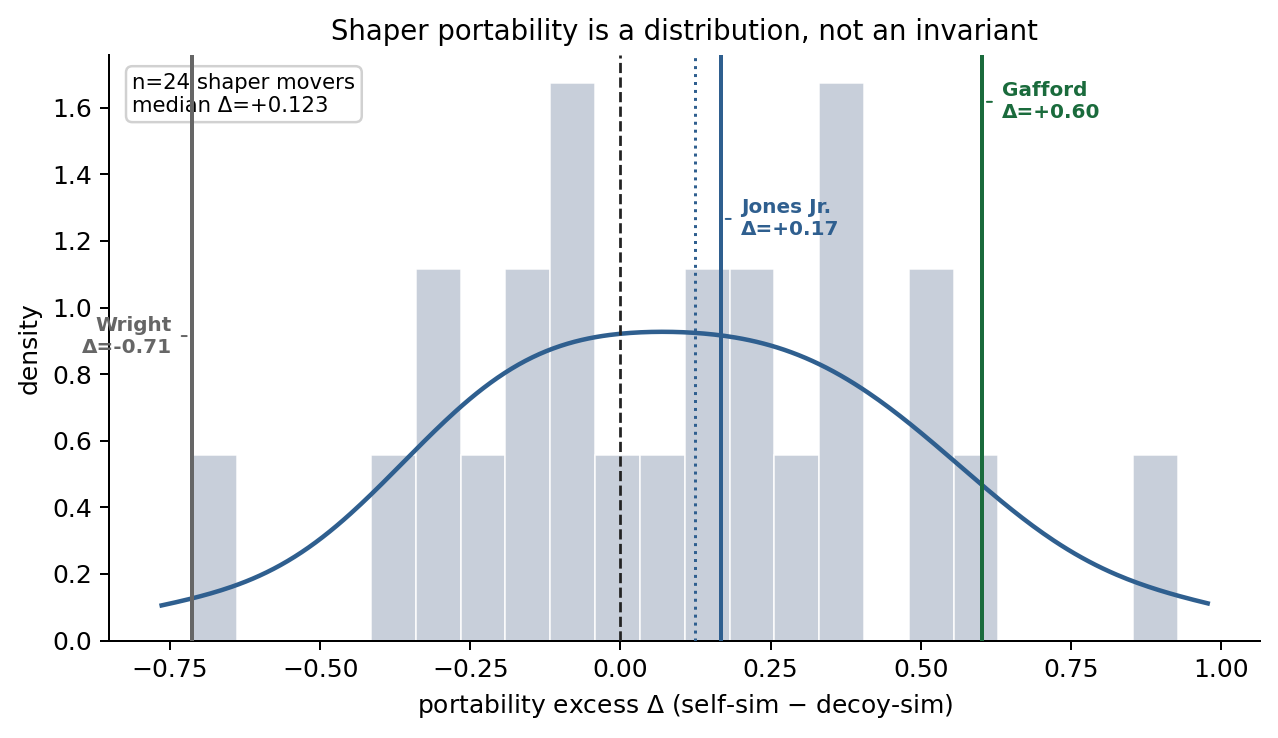
\includegraphics[width=0.92\textwidth]{fig_shaper_delta_dist.png}
 \caption{\textbf{Portability is a distribution, not an invariant.} Realized portability
 $\Delta$ among \textsc{Shaper} movers ($n=24$). Positive $\Delta$ means the player's
 origin structural footprint predicts his destination footprint better than a profile-matched
 decoy's. Endpoints illustrate the distribution; they are not the story.}
 \label{fig:shaper-dist}
\end{figure}

\begin{figure}[H]
 \centering
 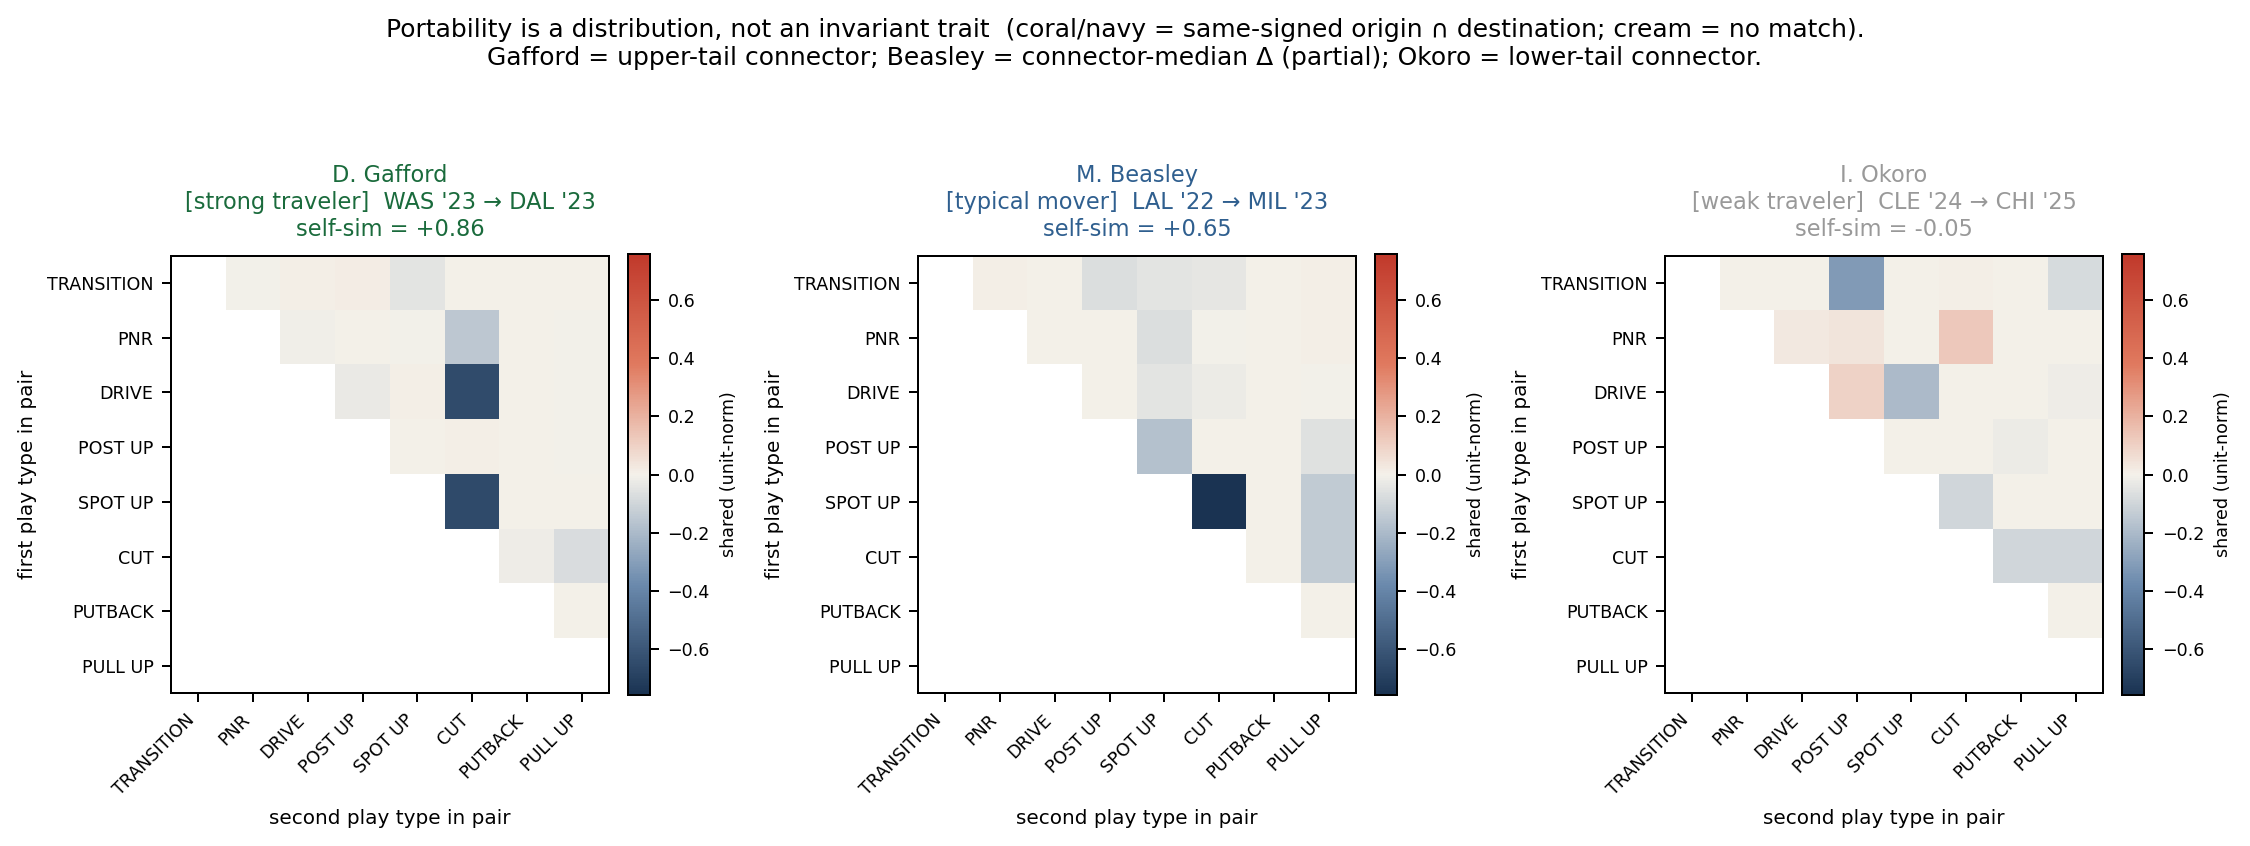
\includegraphics[width=\textwidth,height=0.42\textheight,keepaspectratio]{fig5b_signatures.png}
 \caption{\textbf{Depth of concordance, not a success/failure binary.}
 Each panel is a concordance of origin and destination displacement signatures
 (Eq.~\ref{eq:signature}), not two raw heatmaps side by side. A cell is colored only when
 both teams agree on the sign of that play-type-pair shift when the player is removed:
 navy $=$ shared weakening of the link, coral $=$ shared strengthening, cream $=$ no
 same-sign match. Intensity is shared strength after unit-normalizing each signature.
 Self-sim (panel title) is the cosine of the full signatures; it (not cell count) ranks
 the panels. Sparse/deep concordance (Gafford) outranks many weaker mixed-sign matches
 (Jones Jr.); Wright shows little portable structure. The figure shows whether the same
 player's removal disrupts similar relationships across contexts, not career outcomes.}
 \label{fig:portability}
\end{figure}

\begin{table}[t]
\centering\small
\caption{Shaper distribution endpoints and median contrast (confirmatory sample;
illustrations, not independent evidence). All three rows are \textsc{Shaper}. Init.\
share $u$ is the graph-native initiation share (Eq.~\ref{eq:resid}). Influence and $u$ are
origin-side mover stints used in T1 (for Gafford: partial WAS 2023--24 pre-trade). $\Delta$ is
the profile-matched signature excess (Eq.~\ref{eq:portability}).}
\label{tab:cases}
\begin{tabular}{llccccl}
\toprule
Case & Player & Init.\ $u$ & Influence (o$\to$d) & self-sim & $\Delta$ & Portable \\
\midrule
Strong shaper & D.\ Gafford & 0.036 & $0.335\to0.007$ & $+0.86$ & $+0.60$ & \textbf{Yes} \\
Near shaper median & D.\ Jones Jr. & 0.030 & $0.025\to0.014$ & $+0.21$ & $+0.17$ & \textbf{Yes} \\
Weak shaper & D.\ Wright & 0.016 & $0.030\to0.002$ & $-0.66$ & $-0.71$ & \textbf{No} \\
\bottomrule
\end{tabular}
\end{table}

\paragraph{Does destination context explain the variation?}
Having established heterogeneity (Fig.~\ref{fig:shaper-dist}), the natural front-office
hypothesis is that \emph{fit} decides: wiring ability reappears if the new roster has a hole
for it, and fails if an incumbent already occupies that organizational slot. This paper tests that with
$\text{fit\_score}(p)=-\text{decoy\_sim}(p)$ (Eq.~\ref{eq:fit}), the same profile-matched
decoys as Eq.~\ref{eq:portability}, signed so that high fit means no destination incumbent
already looks structurally like $p$. A minutes-weighted crowding variant checks whether
unweighted decoys diluted a true blocker.
\begin{equation}
\label{eq:fit}
\text{fit\_score}(p) \;=\; -\text{decoy\_sim}(p).
\end{equation}

\emph{Result.} Among shaper movers ($n=24$), fit does not predict signature excess:
$\operatorname{corr}(\text{fit\_score},\Delta)\approx -0.09$;
$\operatorname{corr}(\text{fit\_score},\mathbb{1}[\Delta>0])\approx -0.39$. The
high-travel/high-fit cell is not enriched ($33\%$ portable, $n=6$, vs.\ $58\%$ base rate).
Crowding does not repair the null. Destination hole, as measured from initiation
structure, is not what makes glue-guy roles travel. That is a precise null on
Eq.~\ref{eq:fit}, not a claim that every notion of scheme fit is irrelevant. Checks against
destination-team outcomes (on-court net rating, including origin-to-destination change) are
underpowered and null once corrected for landing-spot quality; those are a different bet.
Origin-side screens are Sec.~\ref{sec:travelfit}.

\subsection{Can organizational function transfer be predicted?}
\label{sec:travelfit}

Section~\ref{sec:portability} established the distribution and the destination-fit null. This
subsection asks whether any origin-side signal separates the upper tail from the lower within
shapers. Named endpoints belong to Fig.~\ref{fig:shaper-dist}; this paper does not re-litigate them.

\paragraph{What was evaluated.}
The target is \emph{role reproduction} (signature excess $\Delta$ / self-similarity), not
wins. Destination vacancy is already null in Sec.~\ref{sec:portability}; the battery asks
what else might separate the upper tail from the lower:
\begin{itemize}[leftmargin=1.6em,itemsep=0.15em]
 \item organizational crowding (minutes-weighted rewrite of Eq.~\ref{eq:fit});
 \item composite travel score (leave-one-out influence + stability + usage);
 \item origin structural influence, usage, and year-to-year signature stability;
 \item play style (cut vs.\ drive origin diet);
 \item position within shapers; origin$\to$destination role transition;
 \item multi-move $\Delta$ consistency;
 \item destination prior-season hub presence, signature shape, move timing, and related
 exploratory candidates (including a $63$-feature destination-side FDR search).
\end{itemize}

\paragraph{Most candidates are null.}
The broader battery does not rescue destination vacancy. The composite travel score is weak
at the population level ($\text{AUC}=0.61$, $\operatorname{corr}=+0.06$ vs.\ self-sim,
$n=294$), and null within shapers as a continuous predictor of $\Delta$ ($r\approx 0$).
Usage, stability, position, role transition, multi-move consistency, and prior-season
destination hub presence do not rescue a within-class rule. Across $63$ destination-side
features, no signal survives Benjamini--Hochberg FDR correction at $q<0.05$ (a small number
of raw $p<0.05$ hits are consistent with chance). Origin cut-share is the only candidate that
shows a consistent directional pattern within shapers, though, as detailed below, it does
not clear conventional significance on its own at this sample size.

\paragraph{The leading (non-significant) candidate: cut-based vs.\ drive-based glue.}
Origin cut share is the most consistent pre-move signal that separates shaper
reproduction among the candidates examined here, but it does not clear conventional
significance as a confirmed within-class screen. On the pre-registered shaper-mover
population ($n=24$), cut share predicts $\Delta$ continuously but not significantly
($\rho=+0.32$, $p=0.13$; rank $\text{AUC}=0.71$, permutation $p=0.041$), and cut-minus-drive
is similarly marginal ($\rho=+0.38$, $p=0.07$). Descriptively, high-cut shapers are
$75\%$ portable (median $\Delta=+0.196$); low-cut shapers are $37.5\%$ portable (median
$\Delta=-0.061$). The effect is still more shaper-specific than not: within-class
$\operatorname{corr}(\text{cut},\Delta)$ is $+0.32$ for shapers vs.\ $+0.12$
(organizers), $+0.06$ (terminals), $+0.10$ (role occupants), though the shaper estimate
itself is not individually significant. Partial correlations controlling for signature
concentration/norm, initiation share, and origin influence/usage jointly are consistent in sign
and similar in magnitude to the raw estimate ($r=+0.34$ to $+0.39$, $p=0.06$--$0.11$), and a
one-move-per-player bootstrap (removing duplicate-mover clustering) keeps $\rho>0$ in
$100\%$ of $2{,}000$ resamples (median $\rho=+0.39$). Dropping the top-three $\Delta$ movers
weakens the estimate further ($\rho=+0.22$, $p=0.33$, $\text{AUC}=0.70$), and only one of two
temporal halves clears a minimum sample size. This paper reads cut-share as a directionally
consistent but underpowered candidate rather than a confirmed screen: at $n=24$ the tercile
contrast is descriptively large, but the continuous tests needed to report it as a confirmed
within-shaper rule do not pass.

Descriptive (not a second classifier): high-cut portable cells include Hayes ($37\%$ cut),
Eubanks ($37\%$), Metu ($32\%$), and Mamukelashvili ($22\%$);
drive-heavier non-portable contrasts include Delon Wright
(Sec.~\ref{sec:portability} lower-tail endpoint) and Evan Fournier ($16\%$ drive,
$\Delta=-0.16$). Cut diet is a screen, not a sufficient condition.

\paragraph{What the search contributes.}
Under these operationalizations, destination vacancy and ``buy the high-influence glue guy'' are the
wrong places to start. Origin cut vs.\ drive diet is the leading directional candidate within
shapers, but it is exploratory relative to the pre-registered portability test, modest
($\sim\!10\%$ of within-shaper rank variation in $\Delta$), and not statistically confirmed
at $n=24$. What the initiation graph cannot see is taken up in Section~\ref{sec:discussion}.

%=============================================================================
\section{Discussion}
\label{sec:discussion}

\paragraph{The instrument, not the first finding.}
Before this paper, offensive organization was largely coaching intuition. After it, it is
measurable. That changes \emph{what questions can be asked}, not merely which answer the first
efficiency question received. Contribution~A is a scientific instrument:
organizational dependence as network perturbation. Contribution~B is a first confirmatory
pass with that instrument. The lasting contribution is the former.

What the first pass reveals is already informative about player structure.
Organizational
function is not player value (Sec.~\ref{sec:orthogonality}); it is behaviorally real
(Sec.~\ref{sec:behavior}); and it is partly player-associated, transferring imperfectly across
teams (Sec.~\ref{sec:portability}). Players possess a measurable organizational function
that is distinct from talent, manifests in offensive behavior, and is partially
player-associated
rather than entirely determined by team context. Shapers make that
component visible where usage hides it; they are not the paper's sole object. Destination
vacancy under a $63$-feature FDR battery does not explain who reproduces; origin cut vs.\
drive is an exploratory, non-confirmed within-shaper candidate
(Sec.~\ref{sec:travelfit}).

The efficiency null (Sec.~\ref{sec:efficiency}) should be read as a boundary finding, not a
failed test of the instrument. A measurement of organizational structure need not
reproduce the outcomes used to evaluate players: structural dependence is measurable, but
it is not equivalent to offensive efficiency. The disclosed on/off identity test
(Sec.~\ref{sec:identity-resilience}) then supplies the construct-native follow-up:
shaper absence displaces the observed association fingerprint more than
usage-matched role-occupant absence. Efficiency does not move; identity does. That is the
scoped ``so what'' for the shaper class in this paper: organizational continuity under
substitution, not a PPP premium. Because the identity test is post-hoc, it answers the
boundary rather than extending the original confirmatory protocol.

The efficiency boundary established in Section~\ref{sec:efficiency} sharpens into an
asymmetry once organizer accumulation is placed alongside it. Losing a structurally
load-bearing but low-usage player (a shaper) does not measurably harm offensive
efficiency: this null holds under possession-level controls, lineup-level talent
adjustment, and a held-four-fixed swap-in design that isolates the marginal contribution of
the fifth player. Organizer accumulation, by contrast, is the one term in this analysis that
moves points per possession robustly and consistently ($+2.35$ pts/$100$,
Table~\ref{tab:coverage}). The contrast suggests that what makes a player offensively
valuable in points is not organizational centrality, shapers are, by construction,
the class this instrument identifies as load-bearing, but replaceability: NBA rosters and coaching
staffs appear well-equipped to reallocate responsibility among shaper-type personnel
without cost, while high-usage organizational talent is not similarly substitutable.
Structural influence identifies who an offense's current wiring depends on; it does not identify
who the offense cannot afford to lose.

\paragraph{What becomes measurable now: from players to teams.}
The framework is not only about individuals. Structural influence is a team-level distribution,
not just a player-level score, and its \emph{concentration} across a roster remains a
natural candidate for organizational resilience at the \emph{team} level: two offenses can
score identically and still differ in how much they depend on one or two load-bearing
players. The player-level on/off identity result (Sec.~\ref{sec:identity-resilience}) is
evidence that such dependence is ecologically real under substitution; elevating roster
influence concentration to a confirmatory team-brittleness claim is still future work.

With a reproducible measure of offensive wiring, researchers and practitioners can ask
questions that previously had no quantitative handle, at both the player and team level:
\begin{itemize}[leftmargin=1.6em,itemsep=0.1em]
 \item Which teams are structurally brittle, and to whose absence specifically?
 \item Which injury would force the largest offensive reorganization?
 \item Which player replacement requires the least rewiring, holding scoring fixed?
 \item Does a given trade preserve or fundamentally rewire offensive identity?
 \item How do coaching systems differ in structural dependence, not only in outcomes?
 \item How do rookies assume organizational responsibility over time?
 \item How does organizational structure evolve across seasons?
 \item Which defenders most disrupt an opponent's wiring (the inverse perturbation
 question flagged below)?
\end{itemize}
These are decision-relevant questions that do not require showing that shapers are worth
a fixed number of extra points. ``Does this help a team win'' need not route through PPP: a
front office that can identify which absence its system can least afford is using the
instrument for decision support without any claim that structural influence is itself a value
metric. Those questions are the ``so what.'' The empirical findings above are a first map
of the terrain the instrument opens, not the closed list of what it is for.

\paragraph{What remains outside the possession graph.}
Portability is largely unpredictable \emph{given what a possession-initiation graph can
see}. Plausible residual channels include coaching deployment, spatial fit, defensive scheme,
specific on-court partnerships, and signature noise from low initiation volume. An
exploratory panel on ``when to acquire'' (brittleness / multiplier triggers) finds no such
timing rule and reinforces the efficiency boundary (Sec.~\ref{sec:efficiency}).

\paragraph{Future work: the inverse question on defense.}
Everything above is an \emph{offensive} wiring diagram. The graph also carries defensive
on-court lineups, which opens a symmetric question this paper does not answer: which defenders reshape
the \emph{opponent's} offensive wiring the most. That requires its own construct-validity work
before it can be evaluated with the same discipline applied to portability. Preparing a defense
for the offense's measured post-removal play-mix pivot---the practical use of the shift already
documented in Sec.~\ref{sec:behavior}---is treated as an application in
Sec.~\ref{sec:applications}, not as an open measurement problem.

%=============================================================================
\section{Practical Applications}
\label{sec:applications}

Brief implications of having the instrument: subordinate to the measurement claim.
The uses below are \emph{illustrative decision contexts} the framework opens, not
validated decision rules from this paper's confirmatory tests.

\subsection{Front office: decision-relevant questions, not a value premium}
Given a roster, structural influence ranks which player's removal most displaces the measured
season-level structural fingerprint
(Sec.~\ref{sec:emerge}), and the same vectors can compare trade targets or
replacements by how much they preserve versus rewire existing measured identity. That is
organizational identity, not a substitute for value
(Secs.~\ref{sec:orthogonality},~\ref{sec:efficiency}). Destination vacancy is not a travel
predictor under the measures tested here (Sec.~\ref{sec:portability}). Within shapers,
origin cut vs.\ drive diet is a directional, exploratory hit-rate pattern at this sample
size (top cut-share tercile $\approx 75\%$ portable vs.\ bottom $\approx 38\%$;
Sec.~\ref{sec:travelfit}): a scouting prompt, not a confirmed rule.

\subsection{Team construction: organizational resilience}
Influence concentration across a roster is a natural candidate for distinguishing
\emph{brittle} offenses from \emph{resilient} ones (Sec.~\ref{sec:discussion}). Two teams
can score identically and still differ sharply on that axis.

\subsection{Coaching: whose absence rewires the offense}
Structural influence quantifies how much of an offense's identity rests on a player. The
disclosed on/off identity test (Sec.~\ref{sec:identity-resilience}) finds that shaper
absence displaces the measured association fingerprint more than absence of a
usage-matched role occupant, even though shaper presence does not move PPP
(Sec.~\ref{sec:efficiency}). A practical question before an absence: \emph{whose removal
most rotates the team's fingerprint, and how does the wiring reorganize?}

\subsection{Scouting and research: find the wiring first}
Structural influence surfaces players who carry organizer-level influence without finishing volume.
Locating organizational function is step one; any within-class travel screen is secondary
and exploratory. The same instrument supports the research questions listed in
Sec.~\ref{sec:discussion}.

\subsection{Coaching: in-game pivots after a removal}
Shaper absence is already associated with a specific, measured shift in offensive play
selection (Sec.~\ref{sec:behavior}): more cuts and pick-and-rolls, fewer spot-ups and drives,
in the disclosed composition tests. That is usable in real time. Once a high-influence player
is out---foul trouble, injury, or a deliberate defensive focus that takes him off the ball---the
offense does not merely lose a body; it pivots toward a known menu. A defense that has mapped
those pivots can change coverage, help responsibilities, and matchup priorities to the structure
the offense is about to become, not only to the player who left. This does not require a new
defender-attribution model; it uses the offensive reorganization the instrument already
measures. The harder inverse question---which defenders most \emph{cause} that rewiring---remains
future work (Sec.~\ref{sec:discussion}).

%=============================================================================
\section{Limitations}
\label{sec:limitations}

\begin{itemize}[leftmargin=1.4em,itemsep=0.2em]
  \item \textbf{Initiation, not within-possession flow.} Edges record who \emph{initiates} each
 play type, not the full pass/screen sequence; intra-possession chains are outside the data.
 \item \textbf{No player tracking.} No spatial data; organizational function is inferred from
 initiation alone: a strength for reproducibility, a limit on mechanism. As a concrete
 illustration of this boundary: Draymond Green, commonly cited as an archetypal offensive
 shaper, classifies as \textsc{Role Occupant / Specialist} (not
 \textsc{Shaper}) in all three sample seasons under Eq.~\eqref{eq:taxonomy}, since
 his organizational contribution is understood to operate primarily through passing and
 communication rather than initiation, both outside what this graph represents.
  \item \textbf{Association, not causation.} Rosters are chosen, not randomized; portability is
 that wiring ability \emph{tends to reappear} (origin-side selection not fully excluded).
 \item \textbf{Small-influence estimation noise.} Near $\resid=0$, taxonomy boundaries are
 approximate for very low-initiation players.
 \item \textbf{Efficiency is a boundary, not the purpose.} The coverage null is a boundary
 finding (Sec.~\ref{sec:efficiency}), not a failed test of the instrument.
 \item \textbf{On/off identity test is disclosed post-hoc.} Sec.~\ref{sec:identity-resilience}
 was not pre-registered; it is a follow-up to the efficiency boundary using a different
 outcome ($D_A$, observed on/off association displacement) from leave-one-out $\load(p)$.
 A prospective replication remains the gold-standard check.
 \item \textbf{Backward-looking by construction.} Origin-side screens extrapolate from what a
 player \emph{has been}, not developmental upside.
 \item \textbf{Cut/drive screen is exploratory and not statistically confirmed.} Directional
 at $n=24$ shaper movers; not part of the pre-registered portability protocol
 (Sec.~\ref{sec:travelfit}). A prospective blind battery on a new season remains the
 gold-standard confirmation; 2025--26 was deliberately excluded from confirmatory tests.
 \item \textbf{Large residual outside the initiation graph.} Most within-shaper $\Delta$
 variation is unexplained after cut/drive; destination context is FDR-null.
 \item \textbf{Fit operationalization.} Destination fit is $-\text{decoy\_sim}$
 (Eq.~\ref{eq:fit}): structural vacancy, not scheme fit or coaching trust.
  \item \textbf{Sample and era.} Three seasons; on-court analyses restricted to the tracking
 subset; median-split thresholds may shift across eras (appendix).
\end{itemize}

%=============================================================================
\section{Conclusion}
\label{sec:conclusion}

Most basketball analytics measure what players produce. This paper introduces a reproducible
graph framework for measuring how they organize production. Offenses are wiring
diagrams, team-level maps of who initiates which play types and whether the same players
jointly hold multiple jobs. Structural influence quantifies each player's contribution to that
organization via network perturbation.

What the instrument reveals in a first confirmatory pass is that organizational function
is distinct from value, visible in play mix, bounded for efficiency, and partly
player-associated (median $\Delta=+0.056$, $n=294$). Low-usage
shaper-type players make that component visible where volume metrics hide it. A disclosed
post-hoc on/off test then finds the construct-native follow-up to the efficiency boundary:
shaper absence displaces offensive identity more than usage-matched role-occupant
absence (Sec.~\ref{sec:identity-resilience}). Destination vacancy is null under the measures
evaluated here; origin cut vs.\ drive diet is exploratory.

The lasting contribution is not a verdict that glue guys raise points per possession, they
do not, at the pre-registered bar. It is that organizational function itself can be
measured, and that its observable stake under substitution is identity, not scoring. That
makes possible a class of reproducible questions, about injuries, trades, development,
coaching systems, resilience, and defensive disruption, that previously existed mostly as
coaching intuition.
Before this paper, offensive organization was hard to study quantitatively. After it, it is
an object of analysis.

%=============================================================================
\appendix
\section{Appendix}
\label{sec:appendix}

\paragraph{A. Threshold sensitivity.} Role assignments (Eq.~\ref{eq:taxonomy}) under
25th/75th-percentile splits, with class-membership stability against the median split.

\paragraph{B. Structural-influence robustness.} Frobenius-distance influence as an alternative to cosine
(Eq.~\ref{eq:load}); within-player influence coefficient of variation across seasons as a stability
check.

\paragraph{C. Portability robustness.} Origin- vs.\ destination-clustered bootstraps, decoy
count $K$ at its pre-registered value, and the permutation null construction
(Sec.~\ref{sec:portability}).

\paragraph{D. Behavioral analyses.} Full within-team play-mix deltas for all four classes and
the route-entropy construction and null (Sec.~\ref{sec:behavior}).

\paragraph{E. Coverage pre-registration.} The complete pre-registered protocol for the
efficiency boundary (Sec.~\ref{sec:efficiency}): feasibility gate, frozen talent control,
fixed-effects specification, and binding no-fallback stop conditions.

\paragraph{F. Structure-only negative analyses.} Additional structure$\to$efficiency attempts
(absence-impact, structural replacement, concentration-vs-defense), each reported as a
registered negative and each reinforcing the efficiency boundary of Section~\ref{sec:efficiency}.

\paragraph{G. Shaper roster (2025--26).} Table~\ref{tab:shaper-appendix} lists every
\textsc{Shaper} player-season in the 2025--26 rotation pool
(Sec.~\ref{sec:emerge}), with the same usage, influence, MPG, and PPG fields reported in
aggregate in Table~\ref{tab:taxonomy}. This is a roster, not a ranking: it is provided for
inspection and replication, not as an endorsement of any individual player's value.

% <<<SHAPER_APPENDIX_BEGIN>>>
\begin{longtable}{llrrrr}
\caption{\textsc{Shaper} players in 2025--26 ($n=41$). Usage is box-score usage rate; influence is $\load(p)$ (Eq.~\ref{eq:load}); MPG and PPG are box-score minutes and points per game. Sorted by team, then influence (descending).}
\label{tab:shaper-appendix}\\
\toprule
Player & Team & Usage & Influence & MPG & PPG \\
\midrule
\endfirsthead
\multicolumn{6}{c}{\tablename~\thetable{} ,  continued} \\
\toprule
Player & Team & Usage & Influence & MPG & PPG \\
\midrule
\endhead
\midrule
\multicolumn{6}{r}{\emph{Continued on next page}} \\
\endfoot
\bottomrule
\endlastfoot
\multicolumn{6}{l}{\textit{BKN}} \\
N. Claxton & BKN & 0.175 & 0.061 & 27.8 & 11.7 \\
J. Wilson & BKN & 0.177 & 0.017 & 15.9 & 6.4 \\
\multicolumn{6}{l}{\textit{BOS}} \\
N. Queta & BOS & 0.145 & 0.170 & 25.3 & 10.2 \\
S. Hauser & BOS & 0.141 & 0.022 & 24.8 & 9.2 \\
\multicolumn{6}{l}{\textit{CHA}} \\
R. Kalkbrenner & CHA & 0.113 & 0.020 & 21.4 & 7.6 \\
M. Diabate & CHA & 0.112 & 0.014 & 26.0 & 7.9 \\
\multicolumn{6}{l}{\textit{DAL}} \\
M. Bagley III & DAL & 0.180 & 0.022 & 20.0 & 10.5 \\
D. Gafford & DAL & 0.151 & 0.016 & 21.7 & 9.5 \\
\multicolumn{6}{l}{\textit{DEN}} \\
T. Hardaway Jr. & DEN & 0.177 & 0.036 & 26.6 & 13.5 \\
C. Braun & DEN & 0.142 & 0.022 & 31.8 & 12.0 \\
C. Johnson & DEN & 0.144 & 0.020 & 30.5 & 12.2 \\
S. Jones & DEN & 0.097 & 0.016 & 22.1 & 5.5 \\
J. Pickett & DEN & 0.148 & 0.014 & 16.1 & 5.2 \\
\multicolumn{6}{l}{\textit{DET}} \\
D. Robinson & DET & 0.152 & 0.044 & 27.4 & 12.2 \\
I. Stewart & DET & 0.164 & 0.017 & 22.7 & 10.0 \\
J. Green & DET & 0.143 & 0.015 & 17.6 & 6.9 \\
\multicolumn{6}{l}{\textit{GSW}} \\
G. Payton II & GSW & 0.177 & 0.033 & 15.6 & 7.5 \\
W. Richard & GSW & 0.123 & 0.019 & 20.0 & 6.4 \\
A. Horford & GSW & 0.163 & 0.016 & 21.5 & 8.3 \\
\multicolumn{6}{l}{\textit{LAC}} \\
B. Lopez & LAC & 0.171 & 0.020 & 21.8 & 8.5 \\
\multicolumn{6}{l}{\textit{LAL}} \\
J. Hayes & LAL & 0.124 & 0.025 & 18.3 & 7.5 \\
\multicolumn{6}{l}{\textit{MEM}} \\
K. Caldwell-Pope & MEM & 0.173 & 0.034 & 21.3 & 8.4 \\
\multicolumn{6}{l}{\textit{MIA}} \\
K. Ware & MIA & 0.174 & 0.352 & 22.1 & 11.1 \\
\multicolumn{6}{l}{\textit{MIL}} \\
J. Sims & MIL & 0.095 & 0.139 & 19.7 & 5.0 \\
A. Green & MIL & 0.135 & 0.025 & 29.1 & 10.4 \\
\multicolumn{6}{l}{\textit{MIN}} \\
R. Gobert & MIN & 0.127 & 0.059 & 31.3 & 10.9 \\
\multicolumn{6}{l}{\textit{NOP}} \\
Y. Missi & NOP & 0.122 & 0.019 & 19.7 & 5.7 \\
\multicolumn{6}{l}{\textit{NYK}} \\
M. Robinson & NYK & 0.102 & 0.233 & 19.6 & 5.7 \\
\multicolumn{6}{l}{\textit{OKC}} \\
I. Hartenstein & OKC & 0.153 & 0.125 & 24.2 & 9.2 \\
I. Joe & OKC & 0.178 & 0.022 & 21.2 & 11.1 \\
A. Caruso & OKC & 0.152 & 0.015 & 18.2 & 6.2 \\
\multicolumn{6}{l}{\textit{ORL}} \\
G. Bitadze & ORL & 0.128 & 0.269 & 15.2 & 5.9 \\
J. Carter & ORL & 0.166 & 0.012 & 16.4 & 6.4 \\
\multicolumn{6}{l}{\textit{PHI}} \\
A. Bona & PHI & 0.108 & 0.061 & 17.4 & 4.8 \\
A. Drummond & PHI & 0.143 & 0.013 & 19.5 & 6.4 \\
\multicolumn{6}{l}{\textit{PHX}} \\
M. Williams & PHX & 0.167 & 0.015 & 23.6 & 11.7 \\
\multicolumn{6}{l}{\textit{POR}} \\
R. Williams III & POR & 0.129 & 0.067 & 17.1 & 6.7 \\
D. Clingan & POR & 0.163 & 0.038 & 27.2 & 12.1 \\
\multicolumn{6}{l}{\textit{SAC}} \\
D. Cardwell & SAC & 0.108 & 0.046 & 20.6 & 5.4 \\
\multicolumn{6}{l}{\textit{SAS}} \\
L. Kornet & SAS & 0.100 & 0.103 & 21.0 & 6.5 \\
\multicolumn{6}{l}{\textit{TOR}} \\
J. Poeltl & TOR & 0.150 & 0.037 & 25.0 & 10.7 \\
\end{longtable}
% <<<SHAPER_APPENDIX_END>>>

\paragraph{H. Play-type inferrer from public play-by-play.}
\label{sec:appendix-inferrer}
No Synergy, Second Spectrum, or tracking feed is used. Possession labels are inferred from
NBA Stats play-by-play V3 fields available via the public API---principally
\texttt{actionType}/\texttt{subType}, event description text, assist tokens on made shots,
shot distance, and court coordinates---after events are normalized into a possession chain.
A rule-based classifier maps those signals onto nine labels
(\texttt{TRANSITION}, \texttt{PNR}, \texttt{DRIVE}, \texttt{POST\_UP}, \texttt{SPOT\_UP},
\texttt{CUT}, \texttt{PUTBACK}, \texttt{PULL\_UP}, \texttt{OTHER}); association and
structural-influence calculations use the eight initiating types listed in
Sec.~\ref{sec:data}, with residual \texttt{OTHER} possessions excluded from the canonical
set after labeling (and after the foul- and PNR-calibration passes below).

Rules fire in fixed priority (highest first). Table~\ref{tab:inferrer-signals} summarizes the
main PBP$\to$label mappings; confidence scores accompany each rule so downstream gates can
prefer high-signal labels when needed.
\begin{table}[h]
\centering
\caption{Possession classifier: public PBP signals to initiating play type.
PNR rows use assist flags that appear only on made shots unless noted.}
\label{tab:inferrer-signals}
\small
\begin{tabular}{@{}p{0.52\linewidth}p{0.40\linewidth}@{}}
\toprule
PBP signal (\texttt{subType} / text / assist) & Label \\
\midrule
Putback / tip subtypes & \texttt{PUTBACK} \\
Cutting / alley-oop subtypes & \texttt{CUT} \\
Fadeaway, hook, turnaround (or post text) & \texttt{POST\_UP} \\
Running / fast-break subtypes or text & \texttt{TRANSITION} \\
Assisted pull-up or floater (made) & \texttt{PNR} (ball handler) \\
Assisted rim finish $\le 6$ ft, not cut/running (made) & \texttt{PNR} (roll man) \\
Missed unassisted pull-up outside the paint & \texttt{PNR} (low confidence) \\
Driving subtype, no PNR cue & \texttt{DRIVE} \\
Unassisted pull-up / step-back & \texttt{PULL\_UP} \\
Assisted 3PT with no stronger creation cue & \texttt{SPOT\_UP} \\
Foul-ending possession left as \texttt{OTHER} & player-tendency relabel \\
\bottomrule
\end{tabular}
\end{table}

\noindent
The strings ``pick'' and ``screen'' never appear in V3 descriptions, so PNR is never read
off a ball-screen token. It is inferred from assist-plus-subtype/distance rules on makes,
a low-confidence missed-pull-up correction, and the player-level calibration pass already
described in Sec.~\ref{sec:data} (shot-event proxy targets; promotion from
\texttt{PULL\_UP}/\texttt{OTHER}).

\paragraph*{Foul treatment.}
Possessions that end in free throws without a classified shot action often fall through to
\texttt{OTHER} at low confidence. A foul-tendency pass then relabels those
\texttt{OTHER}+foul-ending possessions using the fouled initiator's season primary action
type (drive, post-up, PNR, cut, spot-up, pull-up, or transition), stamped at mid confidence
and marked \texttt{foul\_tendency\_relabeled}. Free-throw-only trips that are not attributable
to a half-court initiation are excluded from half-court efficiency tallies where PPP is
computed. A backward attribution audit recovered $98.6\%$ of remaining foul-ending
\texttt{OTHER} possessions by linking them to the initiating offensive action; correcting
misclassified foul endings shifted play-type PPP by at most $0.007$ points and produced no
play-type ranking changes, so the association-matrix corpus inherits the same labels without
a material sensitivity to that residual.

%=============================================================================
% Bibliography. Replace this thebibliography stub with a .bib + \bibliography
% when finalizing; keys match the \citep calls above.
\begin{thebibliography}{99}
\bibitem[Alagappan(2012)]{alagappan2012positions} M.~Alagappan.
  \emph{From 5 to 13: Redefining the positions in basketball.} MIT Sloan Sports
  Analytics Conference, 2012.
\bibitem[Fewell et~al.(2012)]{fewell2012basketball} J.~H.~Fewell, D.~Armbruster,
  J.~Ingraham, A.~Petersen, and J.~S.~Waters. \emph{Basketball teams as strategic networks.}
  PLoS ONE, 7(11):e47445, 2012.
\bibitem[Lutz(2012)]{lutz2012cluster} D.~Lutz. \emph{A cluster analysis of NBA players.}
  MIT Sloan Sports Analytics Conference, 2012.
\bibitem[Rosenbaum(2004)]{rosenbaum2004apm} D.~T.~Rosenbaum.
  \emph{Measuring how NBA players help their teams win.} 82games.com, 2004.
\bibitem[Sill(2010)]{sill2010winval} J.~Sill. \emph{Improved NBA adjusted +/- using
  regularization and out-of-sample testing.} MIT Sloan Sports Analytics Conference, 2010.
\bibitem[Skinner(2010)]{skinner2010anarchy} B.~Skinner. \emph{The price of anarchy in
  basketball.} Journal of Quantitative Analysis in Sports, 6(1), 2010.
\end{thebibliography}

\end{document}
